%% Results and discussion
%%=========================================

\chapter{Results and Discussion}
\label{ch:results}
This chapter presents the results for the experiments we conducted. Section \ref{sec:accuracy_on_datasets_results} presents the results for the general accuracy each model had on three datasets of increasing size. The results for the experiment with two fonts is presented in Section \ref{sec:handling_of_two_fonts}. In Section \ref{sec:noise_handling} we present results of the {\tt EncDecAtt} model's robustness to induced noise. The final ``stress test'' results are presented in Section \ref{sec:stress_test}, and all the results are discussed in Section \ref{sec:result_discussion}. Finally, in Section \ref{sec:reasoning} we analyze the models in context of our results.

%%=========================================

\section{Accuracy on Datasets}
\label{sec:accuracy_on_datasets_results}
Table \ref{table:accuracy_model_data_sets} contains the accuracy for each model on each of the three datasets of various sizes. The accuracy and loss plots for each test are presented below, showing the progression over the epochs.

\begin{table}[H]
    \centering
    \begin{tabular}{|l|l|l|l|}
        \hline 
                                        & \textbf{Small dataset}          & \textbf{Medium dataset}         & \textbf{Big dataset}            \\ \hline
        {\tt VecRep }                   & 16.80\%                         & 25.14\%                         & 55.01\%                         \\ \hline
        {\tt EncDecReg}                 & 41.20\%                         & 55.52\%                         & 95.49\%                         \\ \hline
        {\tt EncDecAtt}                 & \textbf{92.00\%}                & \textbf{97.16\%}                & \textbf{98.75\%}                \\ \hline
    \end{tabular}
    \captionsetup{justification=centering}
    \caption{Test accuracy for each model on each test set, with the best results for each test set highlighted}
    \label{table:accuracy_model_data_sets}
\end{table}

The {\tt EncDecAtt} model had the best results on all three datasets, with the lowest accuracy of 92\%. Across all three datasets, the model had an accuracy of more than 90\%, and the difference between the best and worst results was less than 7\%. This is in contrast to the {\tt EncDecReg} model, which had low accuracy results for both the small and medium datasets, but high accuracy on the big dataset. The {\tt EncDecReg} model had an accuracy of almost 95.5\%, which is less than 4\% worse than the results for the {\tt EncDecAtt} model. The difference in the accuracy between the {\tt EncDecReg} and {\tt EncDecAtt} model on the medium dataset was more than 40\%, and almost 50\% on the small dataset. The {\tt VecRep} model had consistently lower accuracy than the two other, but almost doubled its accuracy from the medium to the big dataset.

\subsection{VecRep}
\subsubsection{Accuracy and Loss}
\resultplots{fig/results/experiment1/small/vecrep/}{plot_accuracy.png}{plot_loss.png}{result1_small_vecrep}{Accuracy and loss for {\tt VecRep} on small dataset}
\resultplots{fig/results/experiment1/medium/vecrep/}{plot_accuracy.png}{plot_loss.png}{result1_medium_vecrep}{Accuracy and loss for {\tt VecRep} on medium dataset}
\resultplots{fig/results/experiment1/big/vecrep/}{plot_accuracy.png}{plot_loss.png}{result1_big_vecrep}{Accuracy and loss for {\tt VecRep} on big dataset}

The minimal increase in accuracy for all three {\tt VecRep} models across the epochs indicates that the model was unable to learn. The loss values for the tests on the small and medium datasets seem to decrease during the first couple of epochs, while the loss value for the test on the big dataset appears highly erratic.

\newpage
\subsubsection{Confusion Matrix}
\begin{figure}[H]
    \centering
    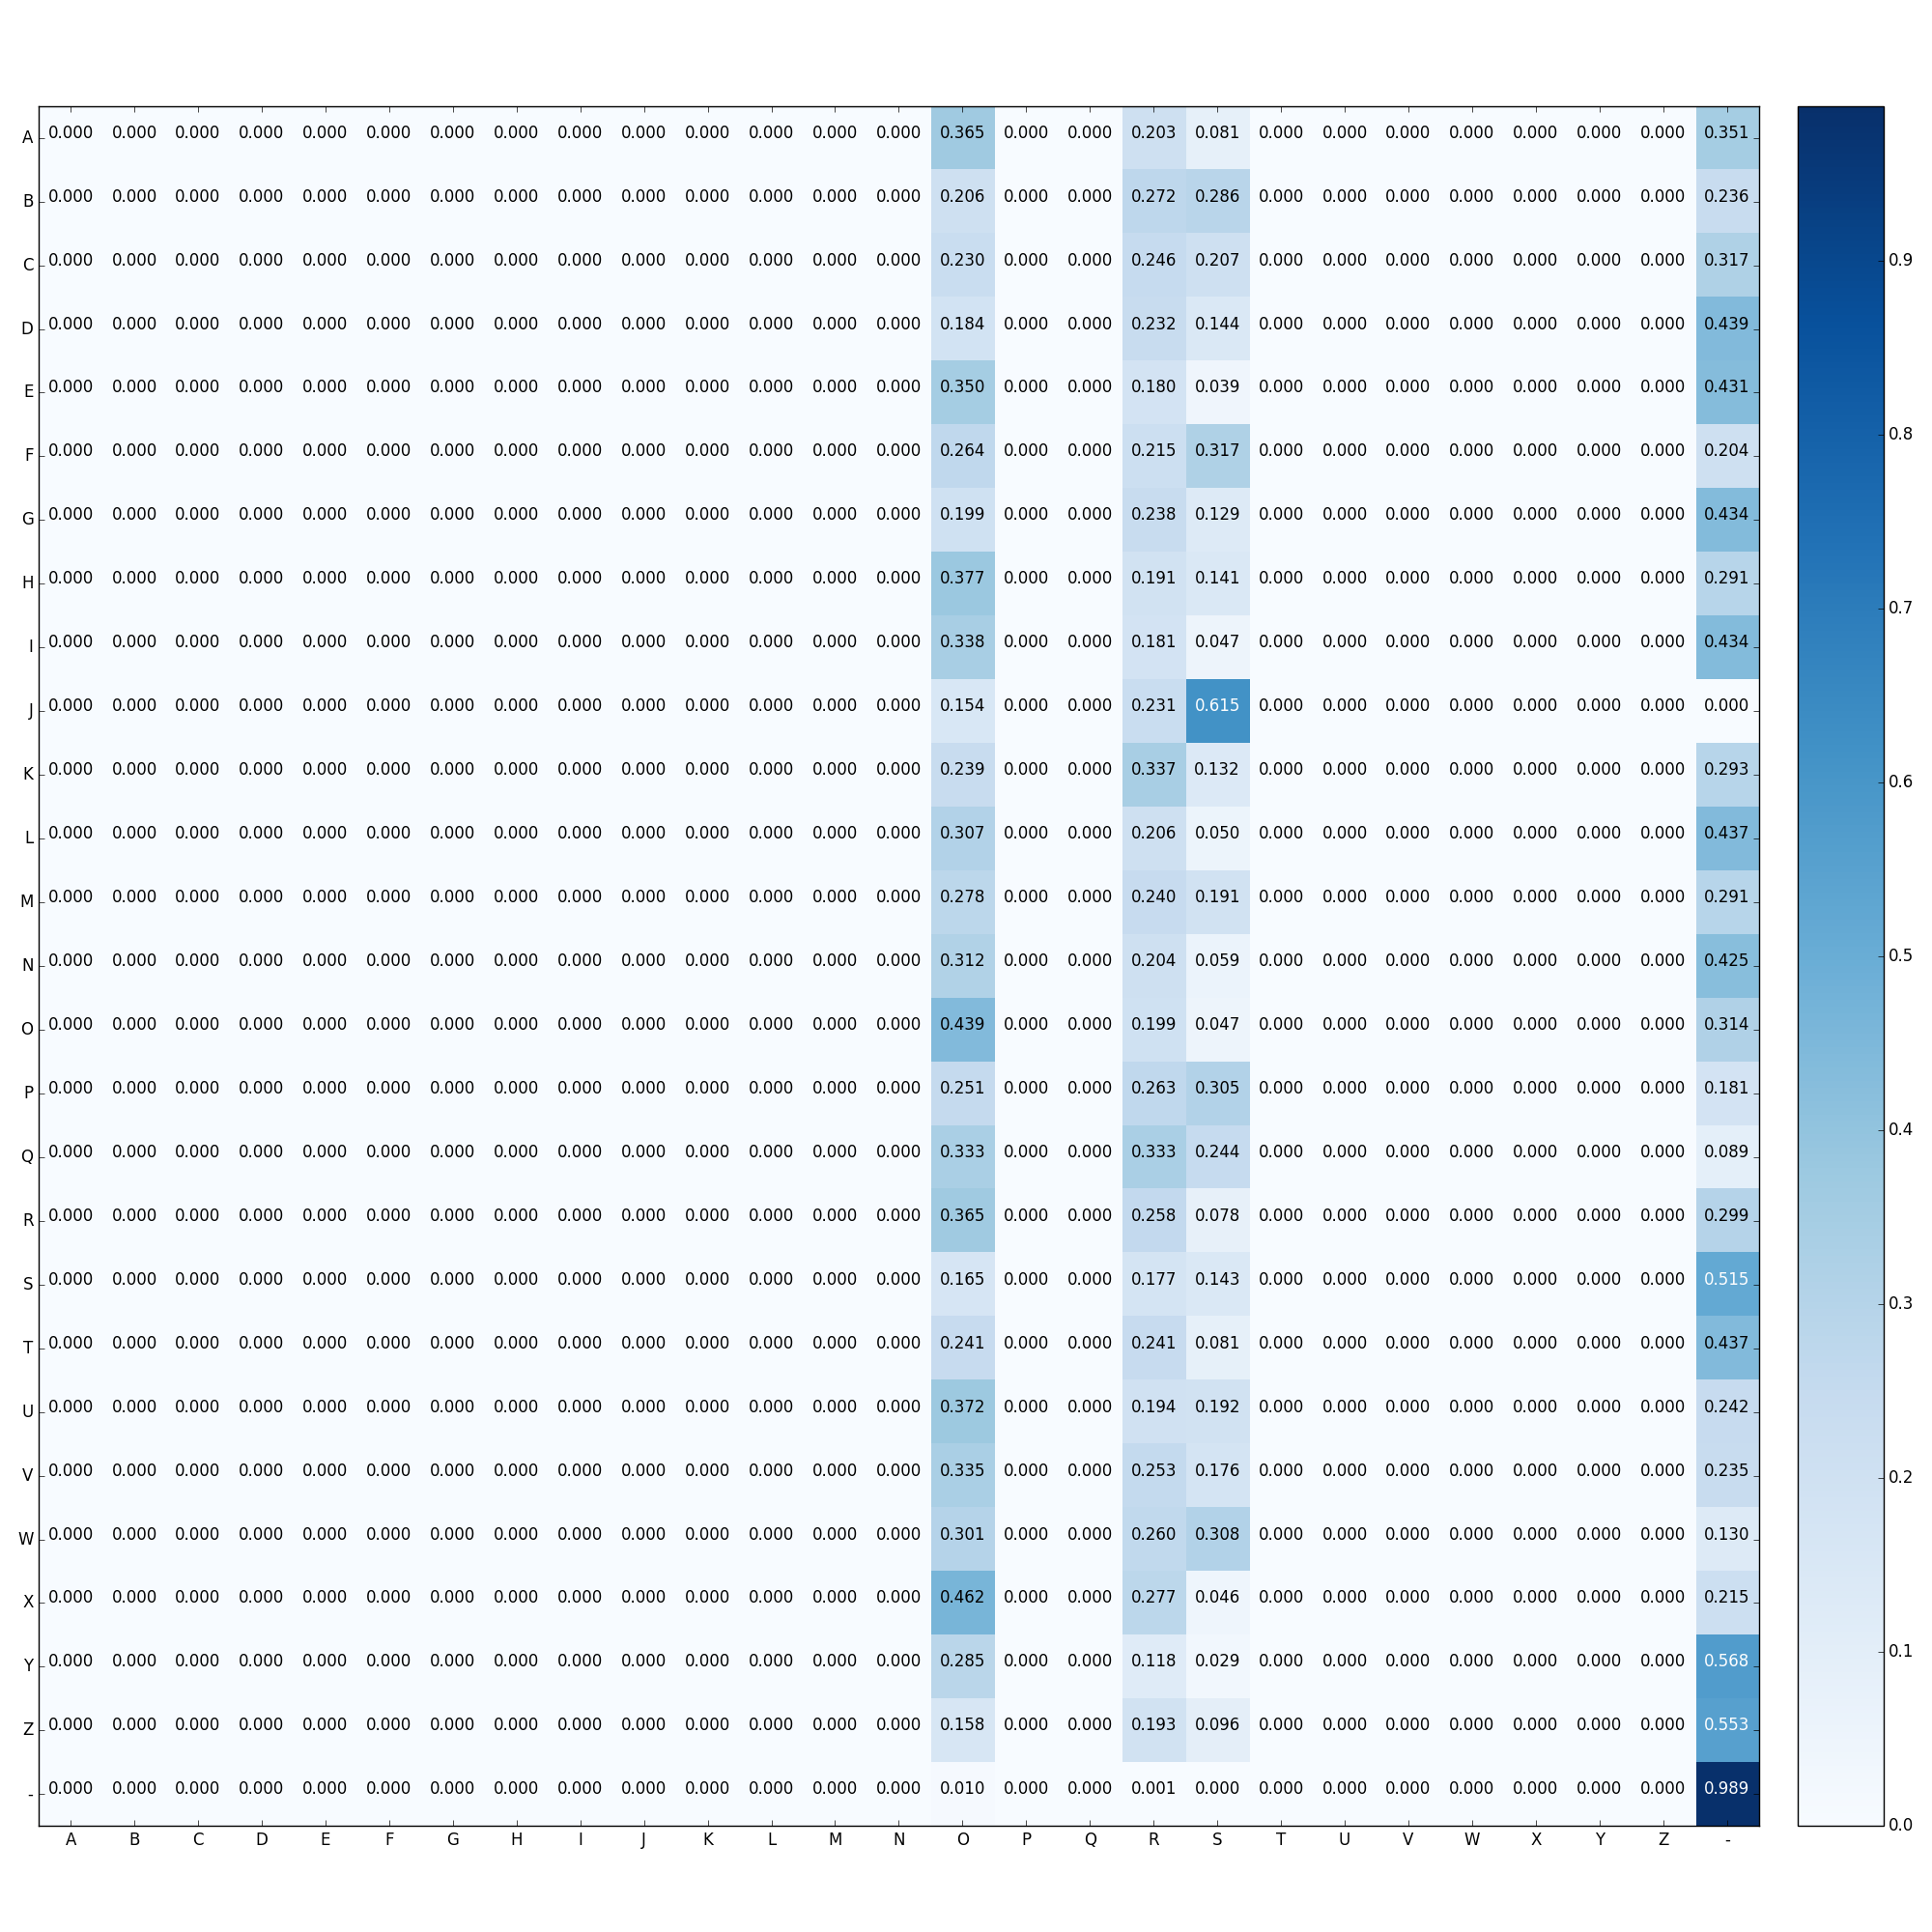
\includegraphics[width=1\textwidth]{fig/results/experiment1/big/vecrep/confusion_matrix.png}
    \caption{Confusion matrix for the best {\tt VecRep} model on the big dataset}
    \label{fig:result1_big_vecrep_confusion_matrix}
\end{figure}

The confusion matrix illustrated in Figure \ref{fig:result1_big_vecrep_confusion_matrix} explains how the {\tt VecRep} model was able to produce an accuracy of over 50\% on the big dataset. The big dataset had a maximum word length of 20 letters, while most words in the English language, as well as in our datasets, are shorter than this. To compensate for this, the labels were zero-padded to fill the empty output labels. The {\tt VecRep} seem to base its predictions on the most common labels, which would be the padding symbol. It also looks to prefer other common labels such as O, R, and S. Every other cell in the confusion matrix is zero, meaning the model did not predict on more than four of the total 27 classes. The confusion matrix clearly indicates that the {\tt VecRep} model was not able to translate between our two constructed languages. 

\subsection{EncDecReg}
\subsubsection{Accuracy and Loss}
\resultplots{fig/results/experiment1/small/encdecreg/}{plot_accuracy.png}{plot_loss.png}{result1_small_encdecreg}{Accuracy and loss for {\tt EncDecReg} on small dataset}
\resultplots{fig/results/experiment1/medium/encdecreg/}{plot_accuracy.png}{plot_loss.png}{result1_medium_encdecreg}{Accuracy and loss for {\tt EncDecReg} on medium dataset}
\resultplots{fig/results/experiment1/big/encdecreg/}{plot_accuracy.png}{plot_loss.png}{result1_big_encdecreg}{Accuracy and loss for {\tt EncDecReg} on big dataset}

The plots for the three best {\tt EncDecReg} models indicates that the models were able to learn. The accuracy for all three of them increase, although the accuracy for the small and medium datasets never improves beyond 60\% accuracy. The loss plots also indicates overfitting, especially on the smallest dataset. The model ran on the biggest dataset seem to improve almost continuously for 400 epochs. This model also had a big spike in the loss values at around epoch 500, but is able to recover after this. These spikes seem to appear with the Adam optimizer when a model is stuck on a plateau and the average of past squared gradients becomes very small, although we are not entirely sure this is the cause.

\newpage
\subsubsection{Confusion Matrix}
\begin{figure}[H]
    \centering
    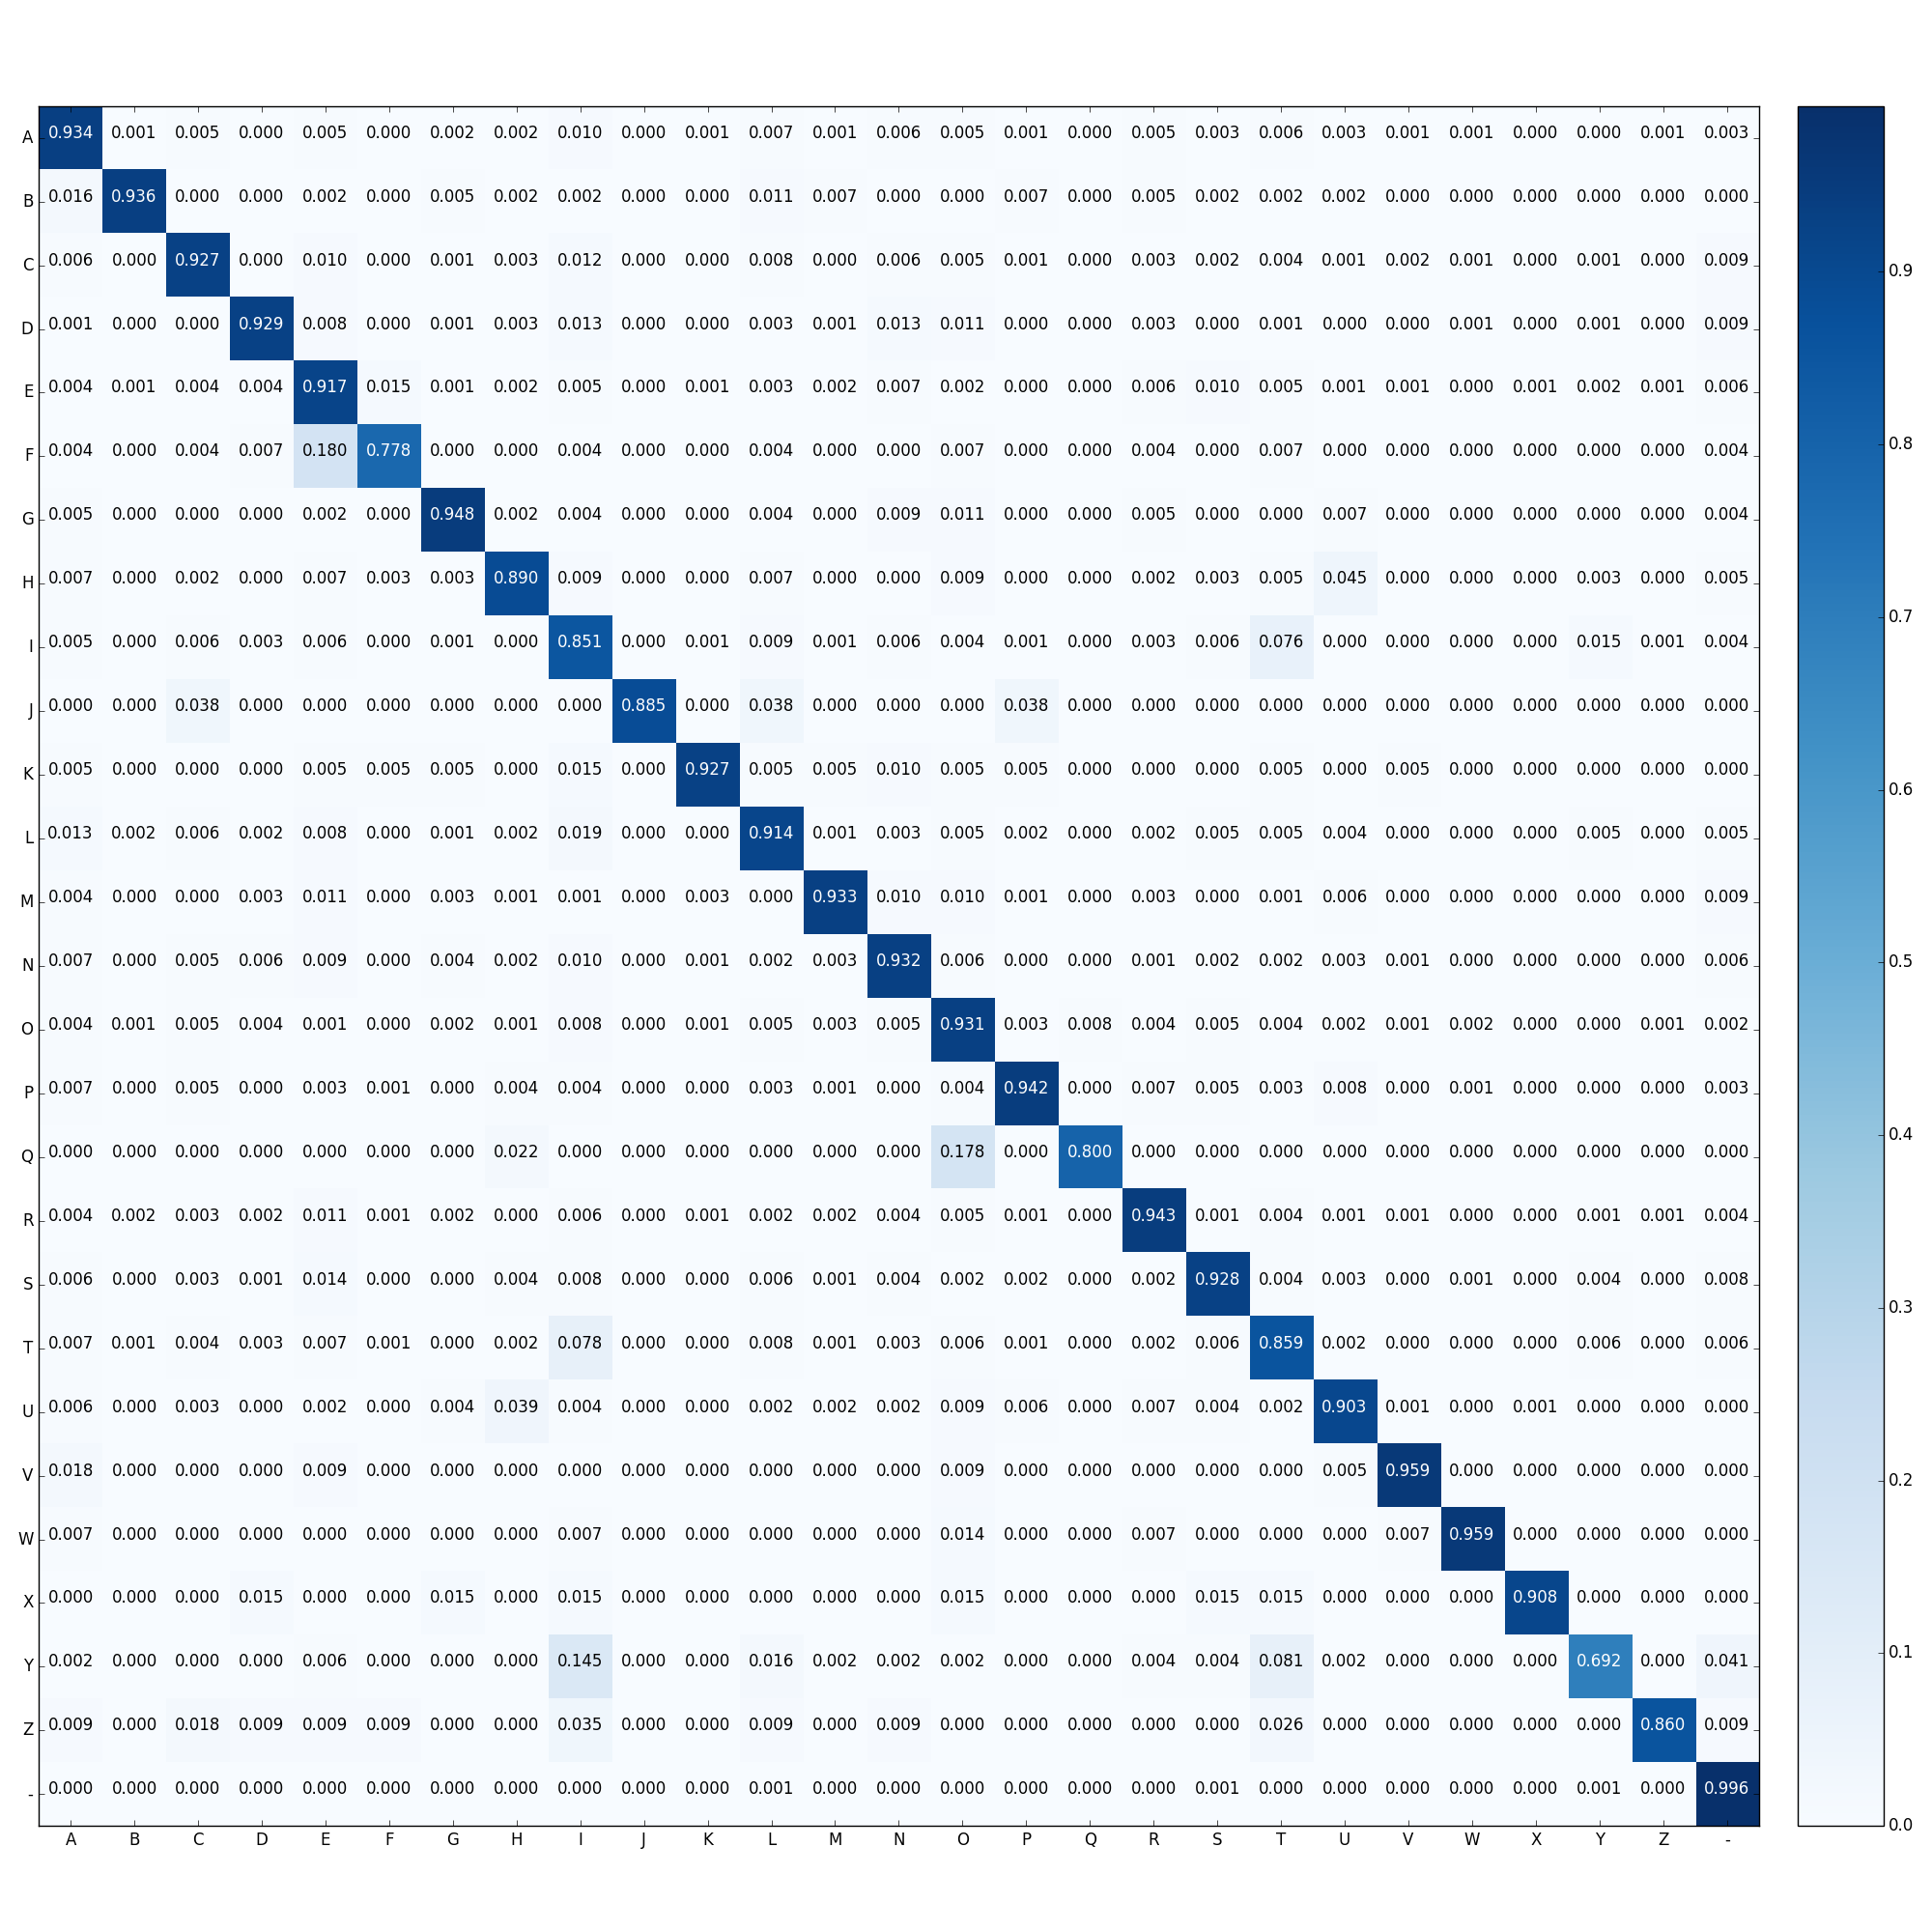
\includegraphics[width=1\textwidth]{fig/results/experiment1/big/encdecreg/confusion_matrix.png}
    \caption{Confusion matrix for the best {\tt EncDecReg} model on the big dataset}
    \label{fig:result1_big_encdecreg_confusion_matrix}
\end{figure}

The {\tt EncDecReg} had an accuracy of almost 95.5\% on the big dataset, which is reflected in the confusion matrix in Figure \ref{fig:result1_big_encdecreg_confusion_matrix}. The confusion matrix has a clearly defined diagonal line with a very high individual accuracy. Most of the labels have an accuracy of over 0.9 with a few exceptions. Y is wrongly labeled as an I in 14.5\% of the instances, and as a T in 8.5\% of the instances. The most wrongly labeled classes are F as an E (18\%) and Q as O (17.8\%).

\subsection{EncDecAtt}
\subsubsection{Accuracy and Loss}
\resultplots{fig/results/experiment1/small/encdecatt/}{plot_accuracy.png}{plot_loss.png}{result1_small_encdecatt}{Accuracy and loss for {\tt EncDecAtt} on small dataset}
\resultplots{fig/results/experiment1/medium/encdecatt/}{plot_accuracy.png}{plot_loss.png}{result1_medium_encdecatt}{Accuracy and loss for {\tt EncDecAtt} on medium dataset}
\resultplots{fig/results/experiment1/big/encdecatt/}{plot_accuracy.png}{plot_lossp.png}{result1_big_encdecatt}{Accuracy and loss for {\tt EncDecAtt} on big dataset}

These plots show much the same as the plots for the {\tt EncDecReg} model. The overfitting is less apparent, although this model also seem to overfit on both the small and medium datasets. The big dataset also have multiple spikes, similar to the {\tt EncDecReg} model. This model also seem to improve for many epochs on the biggest dataset.

\newpage
\subsubsection{Confusion Matrix}
\begin{figure}[H]
    \centering
    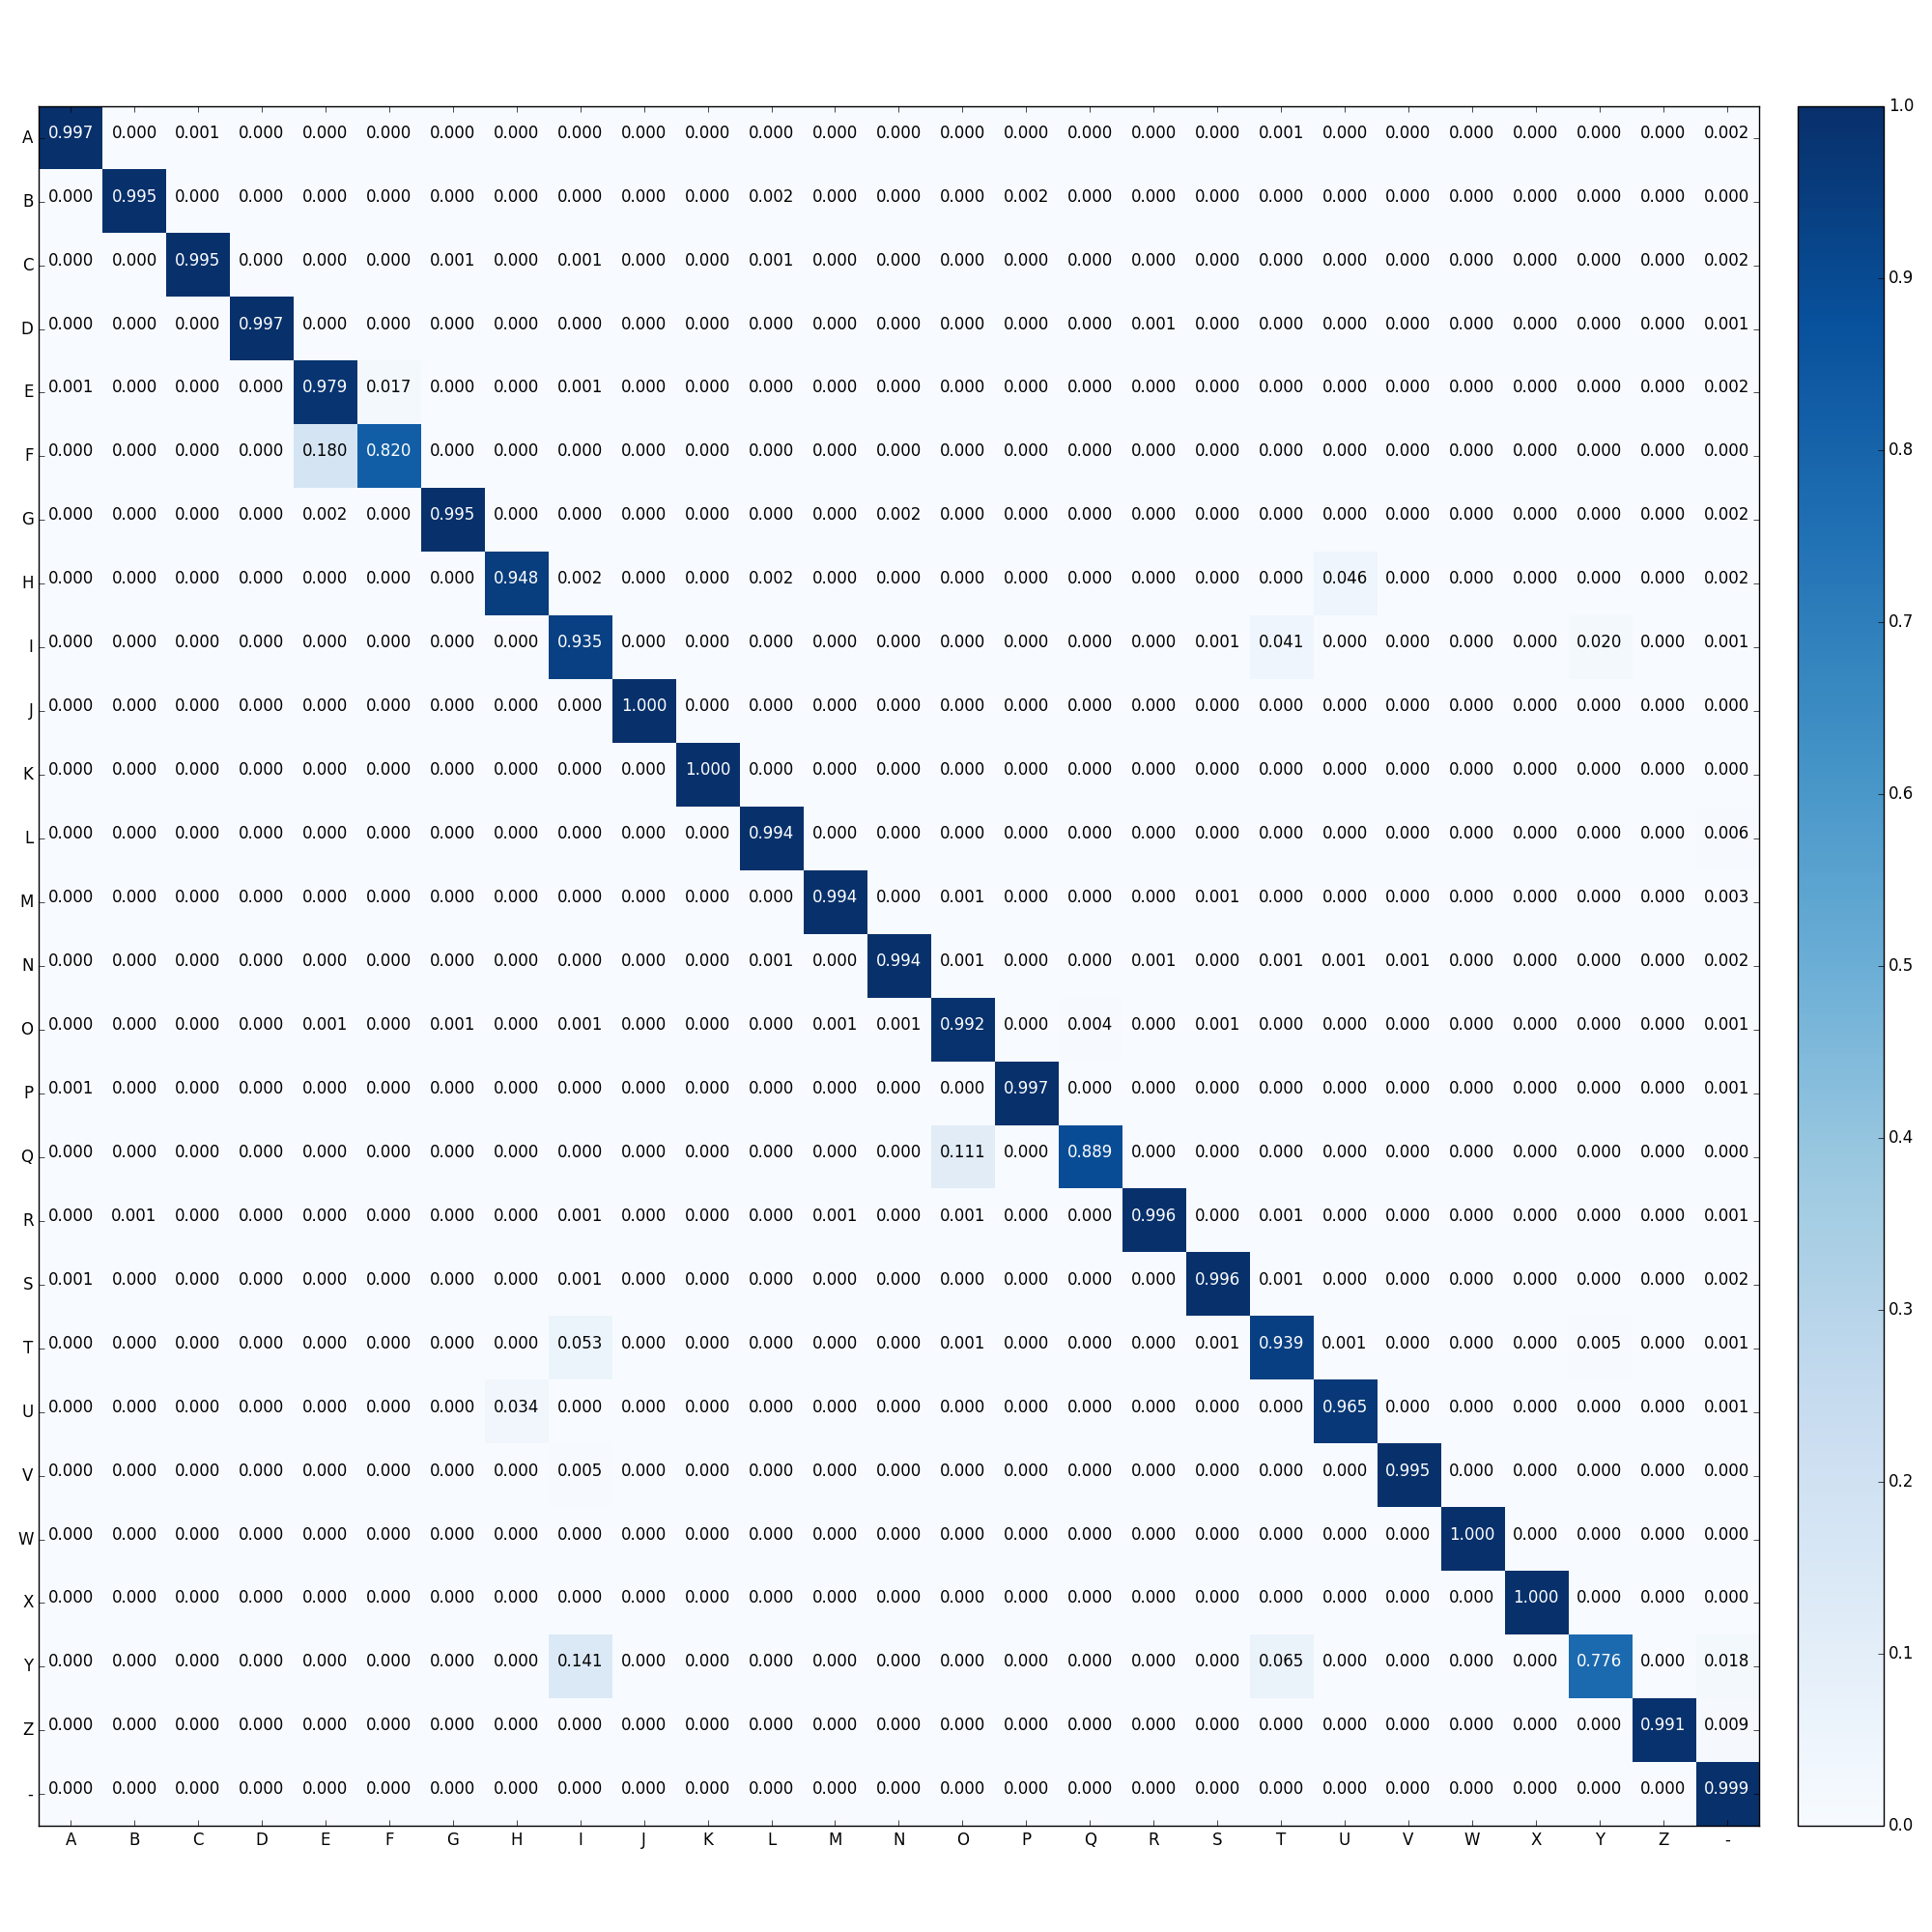
\includegraphics[width=1\textwidth]{fig/results/experiment1/big/encdecatt/confusion_matrix.png}
    \caption{Confusion matrix for the best {\tt EncDecAtt} model on the big dataset}
    \label{fig:result1_big_encdecatt_confusion_matrix}
\end{figure}

The confusion matrix for the {\tt EncDecAtt} model (Figure \ref{fig:result1_big_encdecatt_confusion_matrix}) has high individual accuracy, similar to the results of the {\tt EncDegReg} model, although this model has improved even further. The {\tt EncDegAtt} model successfully classifies four classes without a single error, and only three classes have a lower accuracy than 0.9. However, also this model seem to struggle with some of the same misclassifications as the {\tt EncDegReg} model, namely F as E, Q as O, and Y as I or T.

%%=========================================

\section{Handling of Two Fonts}
\label{sec:handling_of_two_fonts}
Table \ref{table:accuracy_two_fonts} contains the results for each model on the dataset with two fonts. As seen in this table, the accuracy of the {\tt EncDecAtt} is more or less unaffected by the introduction of a second font, whereas the {\tt EncDecReg} and {\tt VecRep} models have reduced accuracy compared to previous experiments. 

\begin{table}[H]
    \centering
    \begin{tabular}{|l|l|}
        \hline 
                                        & \textbf{Accuracy}         \\ \hline
        {\tt VecRep }                   & 40.49\%                   \\ \hline
        {\tt EncDecReg}                 & 88.21\%                   \\ \hline
        {\tt EncDecAtt}                 & 98.93\%                   \\ \hline
    \end{tabular}
    \caption{Accuracy for each model on a dataset with two fonts}
    \label{table:accuracy_two_fonts}
\end{table}

\subsection{Accuracy and Loss For Each Model}
\resultplots{fig/results/experiment2/vecrep/}{plot_accuracy.png}{plot_loss.png}{result2_vecrep}{Accuracy and loss for {\tt VecRep} handling two fonts}
\resultplots{fig/results/experiment2/encdecreg/}{plot_accuracy.png}{plot_loss.png}{result2_encdecreg}{Accuracy and loss for {\tt EncDecReg} handling two fonts}
\resultplots{fig/results/experiment2/encdecatt/}{plot_accuracy.png}{plot_loss.png}{result2_encdecatt}{Accuracy and loss for {\tt EncDecAtt} handling two fonts}

Again the loss plot for the {\tt VecRep} indicates that this model is unable to learn properly, and the loss value seem to worsen after a few couple of epochs. Both the encoder-decoder models seem to overfit.

%%=========================================

\section{Noise Handling}
\label{sec:noise_handling}
Table \ref{table:noise_accuracy} contains the accuracy of the {\tt EncDegAtt} model as the amount of noise was increased. The ``Noise alterations'', e.i. the actual amount of bits altered from a correct 1 to an incorrect 0, or vice versa, is also listed. 

\begin{table}[H]
    \centering
    \begin{tabular}{|l|l|l|}
        \hline 
        \textbf{Noise factor}          & \textbf{Noise alterations}       & \textbf{Accuracy}         \\ \hline
        0\%                            & 0\%                              & 98.06\%                   \\ \hline
        2\%                            & x.xx\%                           & 95.83\%                   \\ \hline
        5\%                            & 2.98\%                           & 93.35\%                   \\ \hline
        6\%                            & 3.46\%                           & 90.93\%                   \\ \hline
        8\%                            & 4.45\%                           & xx.xx\%                   \\ \hline
        10\%                           & 5.46\%                           & 69.36\%                   \\ \hline
        15\%                           & 7.94\%                           & 66.77\%                   \\ \hline
        20\%                           & 10.41\%                          & 59.51\%                   \\ \hline
        40\%                           & 20.32\%                          & 47.67\%                   \\ \hline
        50\%                           & 25.28\%                          & 46.20\%                   \\ \hline
        60\%                           & 30.18\%                          & 45.29\%                   \\ \hline
    \end{tabular}
    \caption{Accuracy for the {\tt EncDecAtt} model}
    \label{table:noise_accuracy}
\end{table}

\begin{figure}[H]
    \centering
    \captionsetup{justification=centering}
    \begin{tikzpicture}
        \begin{axis}[
            xmin=0, xmax=60,
            ymin=0, ymax=1,
            minor y tick num={5},
            minor x tick num={1},
            ylabel=accuracy,
            xlabel=noise,
        ]
            \addplot[draw=red] table[x index=0,y index=1,col sep=comma]{data/noise.csv};
        \end{axis}%
    \end{tikzpicture}%
    \caption{Change of accuracy as the amount of noise is increased}
    \label{fig:noise_accuracy}
\end{figure}

The accuracy is also plotted in Figure \ref{fig:noise_accuracy}, which illustrates how the accuracy deteriorated as the amount of noise was increased. This graph graphically illustrates how the deterioration of the accuracy first falls fast, then flattens out once the amount of noise gets more and more dominant. As shown in both the table and the graph, the accuracy decreased by less than 1.5\% when the noise was increased from 40\% to 50\%. Similarly, the accuracy decreased with less than a percent when noise was further increased to 60\%. This is in contrast to how the accuracy decreased by almost 5\% when noise was introduces to a perfect dataset compared to a dataset with 5\% noise. Further, the accuracy decreased by 24\% when noise was increased from 5\% to 10\%.

This illustrates the difference in accuracy when learning and predicting on datasets that are perfect, near-perfect, and datasets with significant amounts of noise. It also illustrates that increasing noise on datasets that already have much noise in them have a smaller effect on the accuracy.

%%=========================================

\section{Stress Test}
\label{sec:stress_test}
This experiment was done on the models {\tt EncDecReg} and {\tt EncDecAtt}, as the {\tt VecRep} model already had poor results on the experiment that was significantly simpler.

\begin{table}[H]
    \centering
    \begin{tabular}{|l|l|}
        \hline 
                                        & \textbf{Accuracy}         \\ \hline
        {\tt EncDecReg}                 & 55.02\%                   \\ \hline
        {\tt EncDecAtt}                 & 88.44\%                   \\ \hline
    \end{tabular}
    \caption{Accuracy for each model on the stress test}
    \label{table:accuracy_stress_test}
\end{table}

\subsection{EncDecReg Results}
\begin{figure}[H]
    \centering
    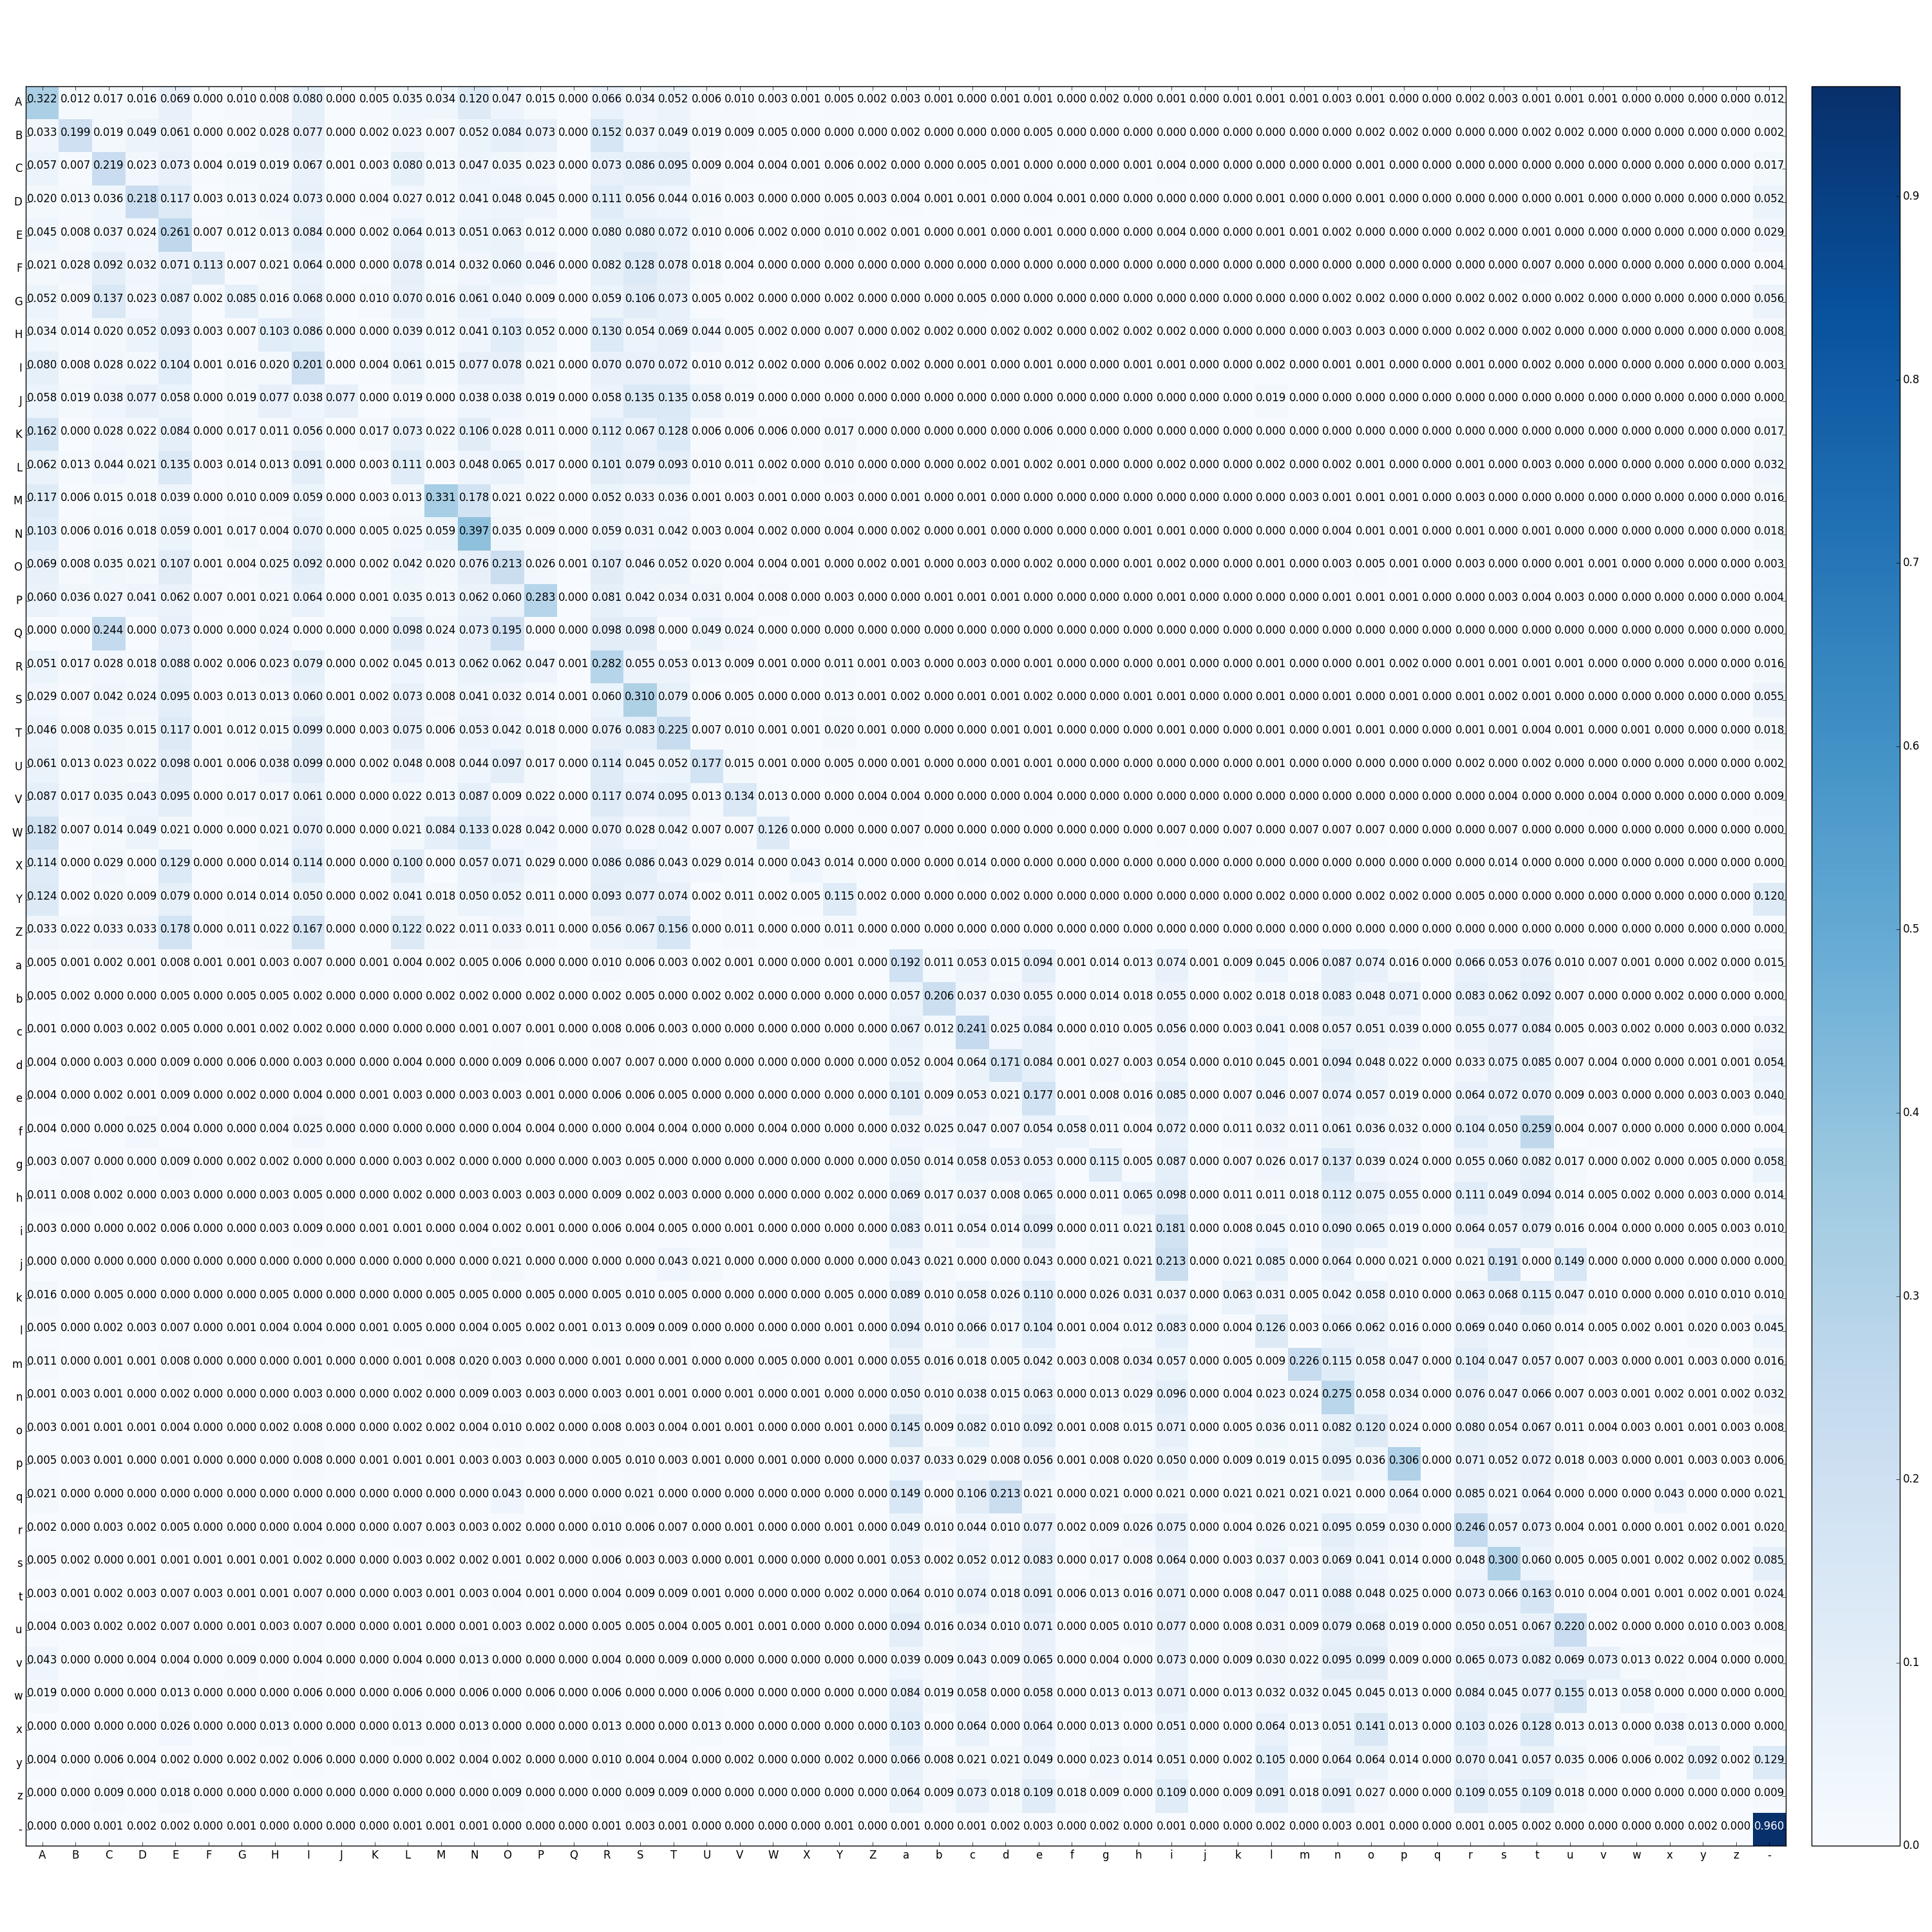
\includegraphics[width=1\textwidth]{fig/results/experiment4/encdecreg/confusion_matrix.png}
    \caption{Confusion matrix for the best {\tt EncDecReg} model on the stress test}
    \label{fig:result4_encdecreg_confusion_matrix}
\end{figure}

Shown in Figure \ref{fig:result4_encdecreg_confusion_matrix} is the confusion matrix for the best {\tt EncDecReg} model on the stress test. As depicted in this matrix, the model had a hard time classifying the labels correctly, which corresponds to its accuracy of 55\%. Despite the somewhat low accuracy, the confusion matrix shows traces of a faint diagonal line going from corner-to-corner, indicating correct classifications. In general, the model seem capable of separating the upper-cased and lower-cased letters from each other, having almost no incorrect labeling shared between the two halves of the matrix. For both groups of upper-cased and lower-cased classes, the model seem to favor a few letters in each, wrongly classifying them across a wide spectrum of other letters.

\subsection{EncDecAtt Results}
\begin{figure}[H]
    \centering
    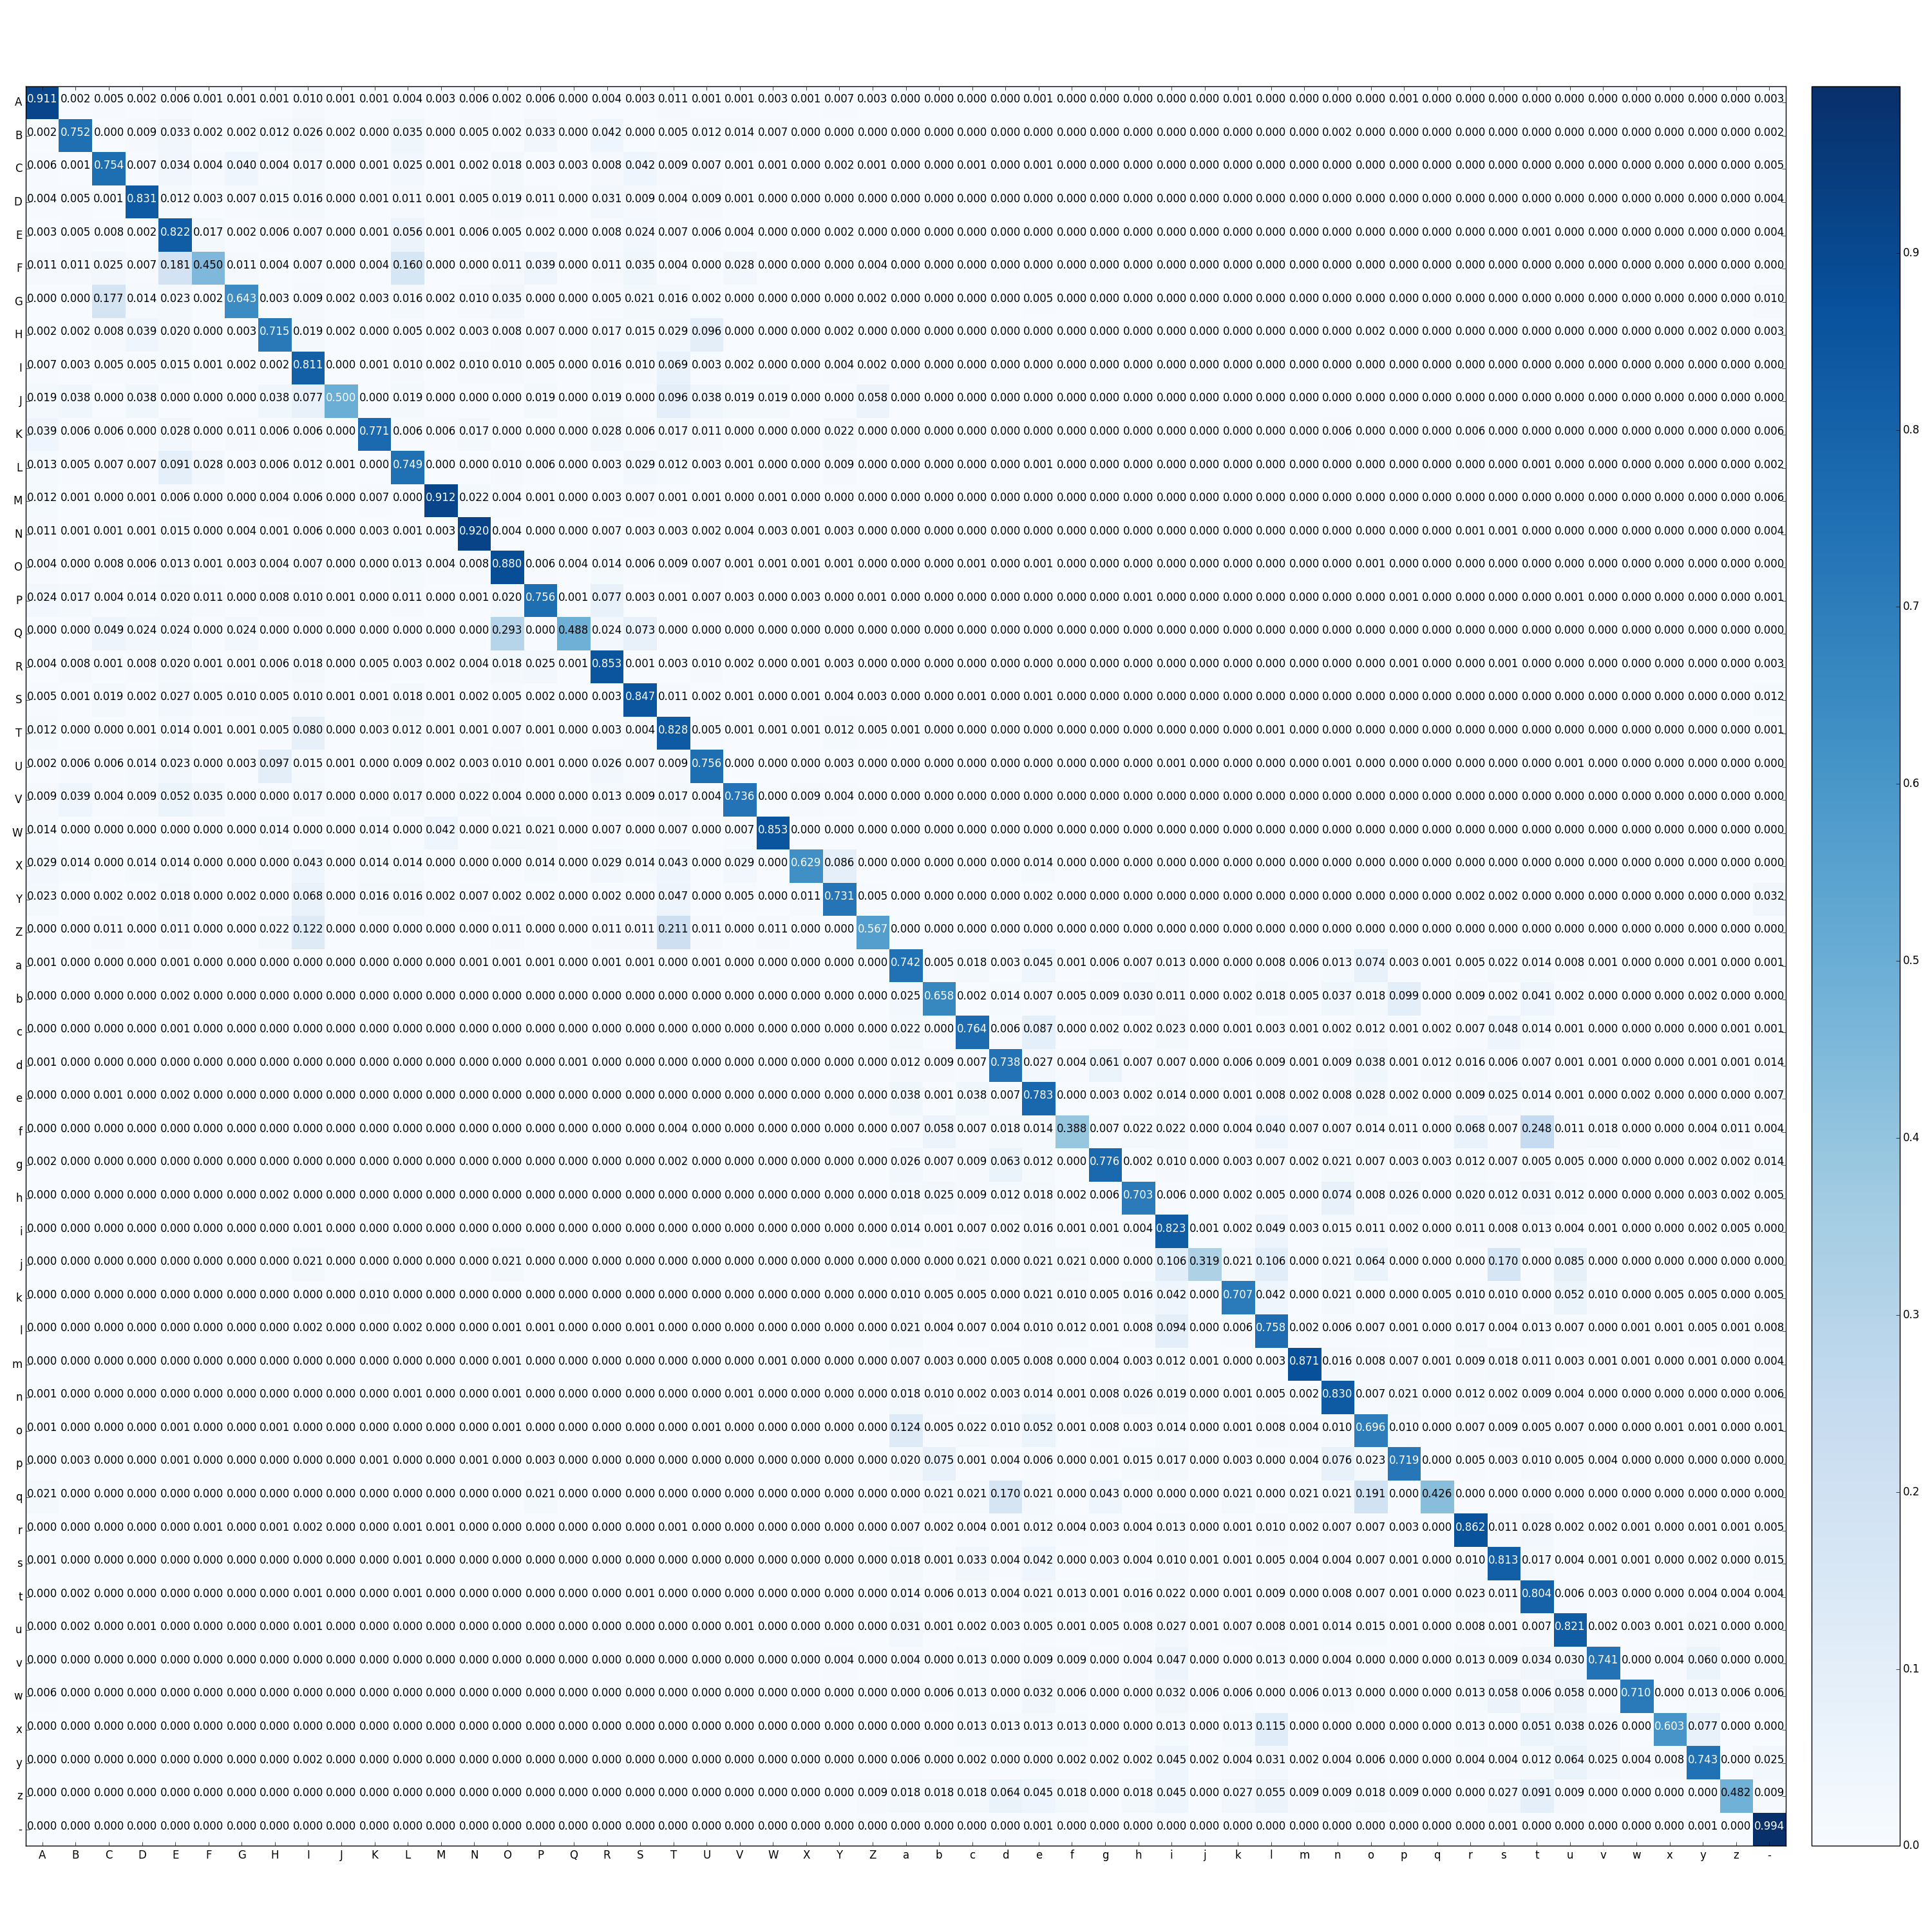
\includegraphics[width=1\textwidth]{fig/results/experiment4/encdecatt/confusion_matrix.png}
    \caption{Confusion matrix for the best {\tt EncDecAtt} model on the stress test}
    \label{fig:result4_encdecatt_confusion_matrix}
\end{figure}

Figure \ref{fig:result4_encdecatt_confusion_matrix} shows the classification matrix of the best {\tt EncDecAtt} model on the stress test. This matrix depicts a clear diagonal line from corner-to-corner, indicating that the model has been able to, for the most part, classifying labels correctly. Although there are certain labels that are misclassified, the vast majority of labels are correctly classified, which corresponds to the accuracy of over 88\% for this model. The confusion matrix also show almost no overlap between the labels in the upper-cased and lower-cased classes, indicating that also this model was able to separate these groups from each other. Some of the labels are repeatably misclassified, and many of these are the same misclassifications we have seen in other tests for the same model.

%%=========================================

\section{Result Discussion}
\label{sec:result_discussion}
In this section, we discuss and compare the various results and models against each other. We also answer the research goals we defined earlier. The final conclusion is given in Chapter \ref{ch:conclusion}.

\subsection{General Discussion}
The first experiment indicated that the {\tt VecRep} model was unable to learn the problem to a satisfactory degree. The confusion matrix indicates that the model is unable to actually translate anything, and relies on classifying the padded values. {\tt EncDecReg} and {\tt EncDecAtt} both show indications that they learned to translate between our two languages, especially when the size of the datasets was increased. At the same time, the {\tt EncDecAtt} model outperformed the {\tt EncDecReg} model in every single experiment. The latter model also reached impressive results for the most complicated experiments we carried out. While the only difference between these two encoder-decoder based models is the attention mechanism, there is a big difference in their performance. We see this both when the datasets are small, and in more complex experiments.

\subsection{Discussion In Terms of Research Questions}

\subsubsection{Ambiguity in Character Signature Sequences}
In our first research question, \textbf{RQ1}, we asked if the models were able to deal with ambiguity in the input data. In our first experiment, we used the same system configurations as shown in Table \ref{table:signature_sequence_example}, which we used to illustrate how some of the letter signatures were either identical or subsequences of another. In this table we showed that the letters C, I, J, L, T, and Y all shared the same unique signature of three black pixels. The other letters that also shared an identical signature were E and F, H and U, O and Q, and S and X. 

Comparing these sets to the confusion matrices, we can see that some of these characters were indeed those the models struggled to classify correctly. Specifically, U, I and T, F and E, as well as Q and O were problematic for both the encoder-decoder models, although their accuracy were no lower than 0.692 for the {\tt EncDegReg} model, and 0.776 for the {\tt EncDegAtt} model on any label. The most commonly wrongly classified label was an E as F, with both the models having an equal confusion of 0.18. 

These numbers indicate that there is still room for improvement, and that ambiguity may be a concern.

\subsubsection{Handling of Multiple Fonts}
Experiments have indicated that both the encoder-decoder models are able to handle more than one font, as questioned in \textbf{RQ2}, although the model without the attention mechanism had visible lower results than experiments carried out on datasets consisting of one font. The {\tt EncDecAtt} model was more or less unaffected by the introduction of an additional font in the first experiment. The same model also yielded good results in the stress test, where the input consisted of five different fonts. On the same test, the {\tt EncDecReg} model had much lower results, indicating that this model may be unsuitable for input with such high variance in the sequences.

\subsubsection{Handling of Noise}
Lastly, \textbf{RQ3} asked if the model(s) were able to adapt to noise and imperfect input data. Experiments have shown that the {\tt EncDecAtt} model was able to handle increasing amounts of noise, although the accuracy decreased as the noise factor increased. For a noise factor of 5\%, the accuracy decreased by a little less than 5\%, while a noise factor of 10\% decreased the accuracy by more than 28\%. With a noise factor of 10\%, every 10th bit may end up corrupted. If this is reasonable to expect in a real-world scenario is hard to say. We have decided to conclude this question by stating that the {\tt EncDecAtt} was able to handle noise in a satisfactory manner.

\subsection{Discussing the Research Goal}
Our goal in this thesis was to create a model that was able to use signature sequences to recognize letters and words in machine written text. The results from our experiments, which has been presented in this chapter, indicates that we were successful in reaching this goal. The two encoder-decoder models, especially the {\tt EncDecAtt}, has been successful in recognizing words with a high accuracy, and we have found these results satisfactory for our evaluation.

%%=========================================

\section{Analysis}
\label{sec:reasoning}
In section we look closer at how the models work and we analyze why we got the results we did. 

\subsection{Encoding}
We have evaluated the encoding mechanism of the encoder-decoder framework. This was done by training a model on a noise induced dataset, and then feeding the same words multiple times with the same amount of noise, but different random seeds. We fed the model three words ten times and plotted the encoded context vector to a low dimensional space using principal component analysis (PCA). 

\begin{figure}[!ht]
    \centering
    \begin{subfigure}{.5\textwidth}
        \centering
        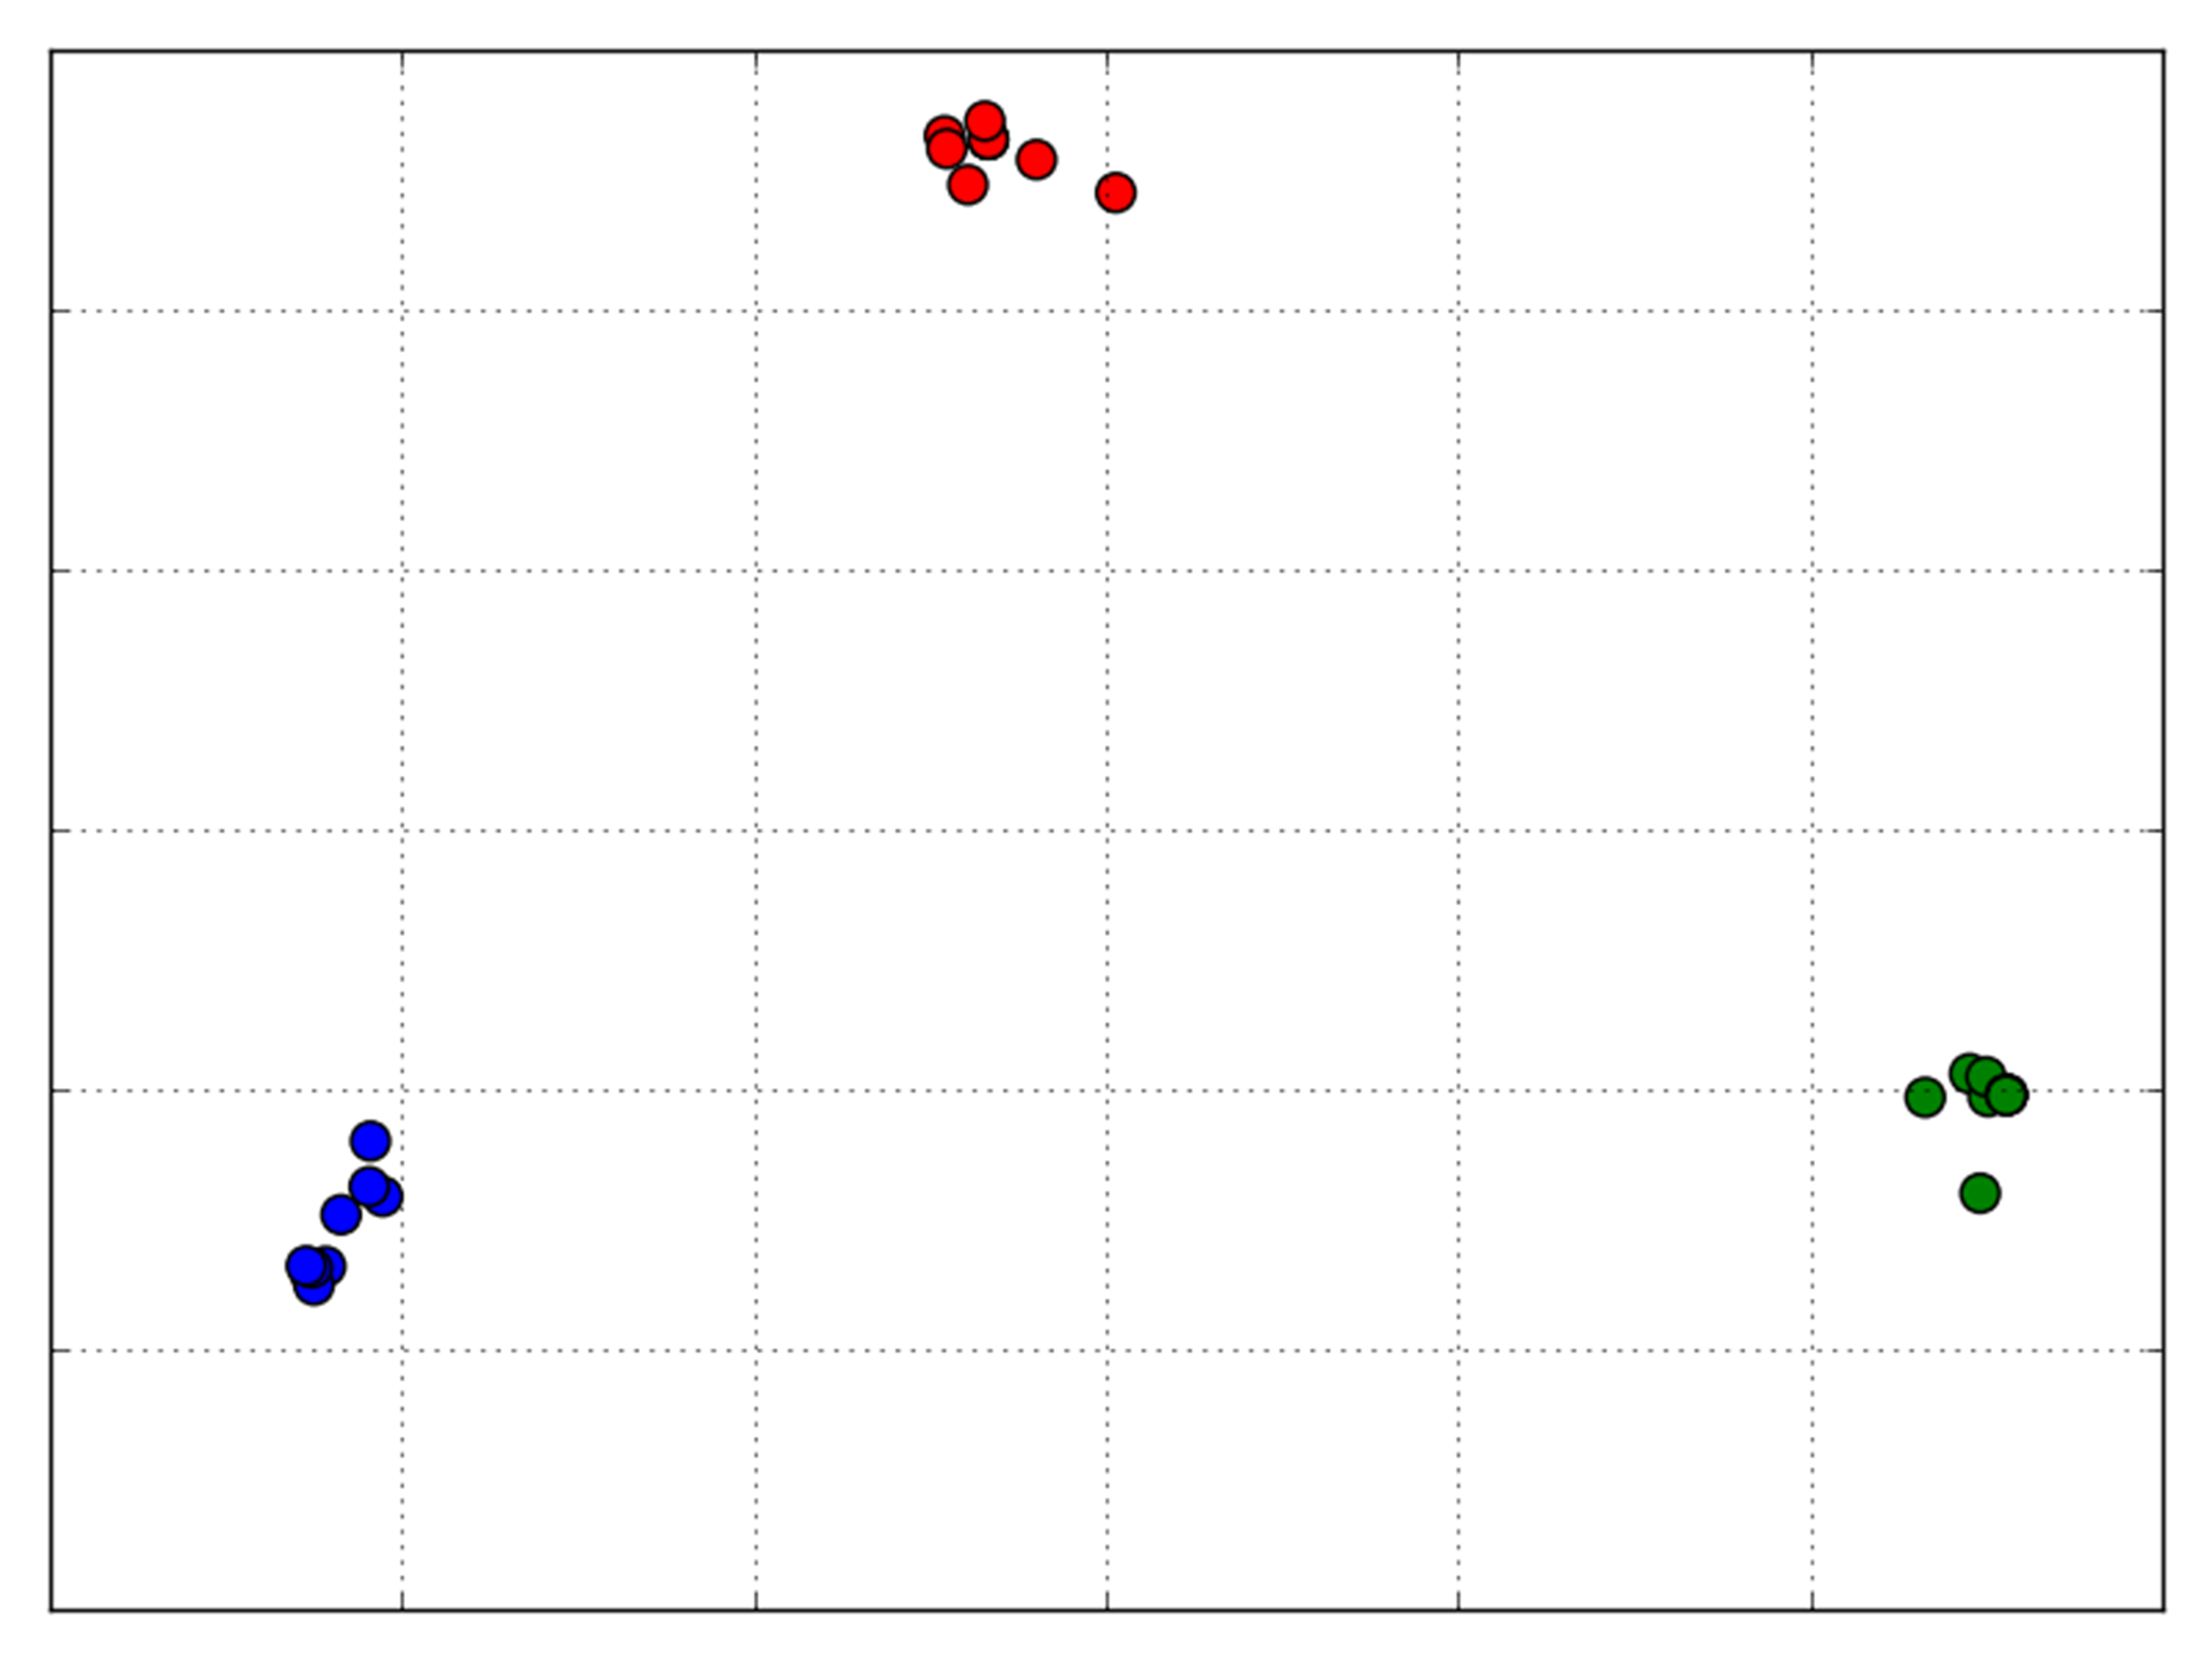
\includegraphics[width=.9\linewidth]{fig/results/context_vector.png}
        \caption{1\% noise}
        \label{fig:context_vector_plot_1}
    \end{subfigure}%
    \begin{subfigure}{.5\textwidth}
        \centering
        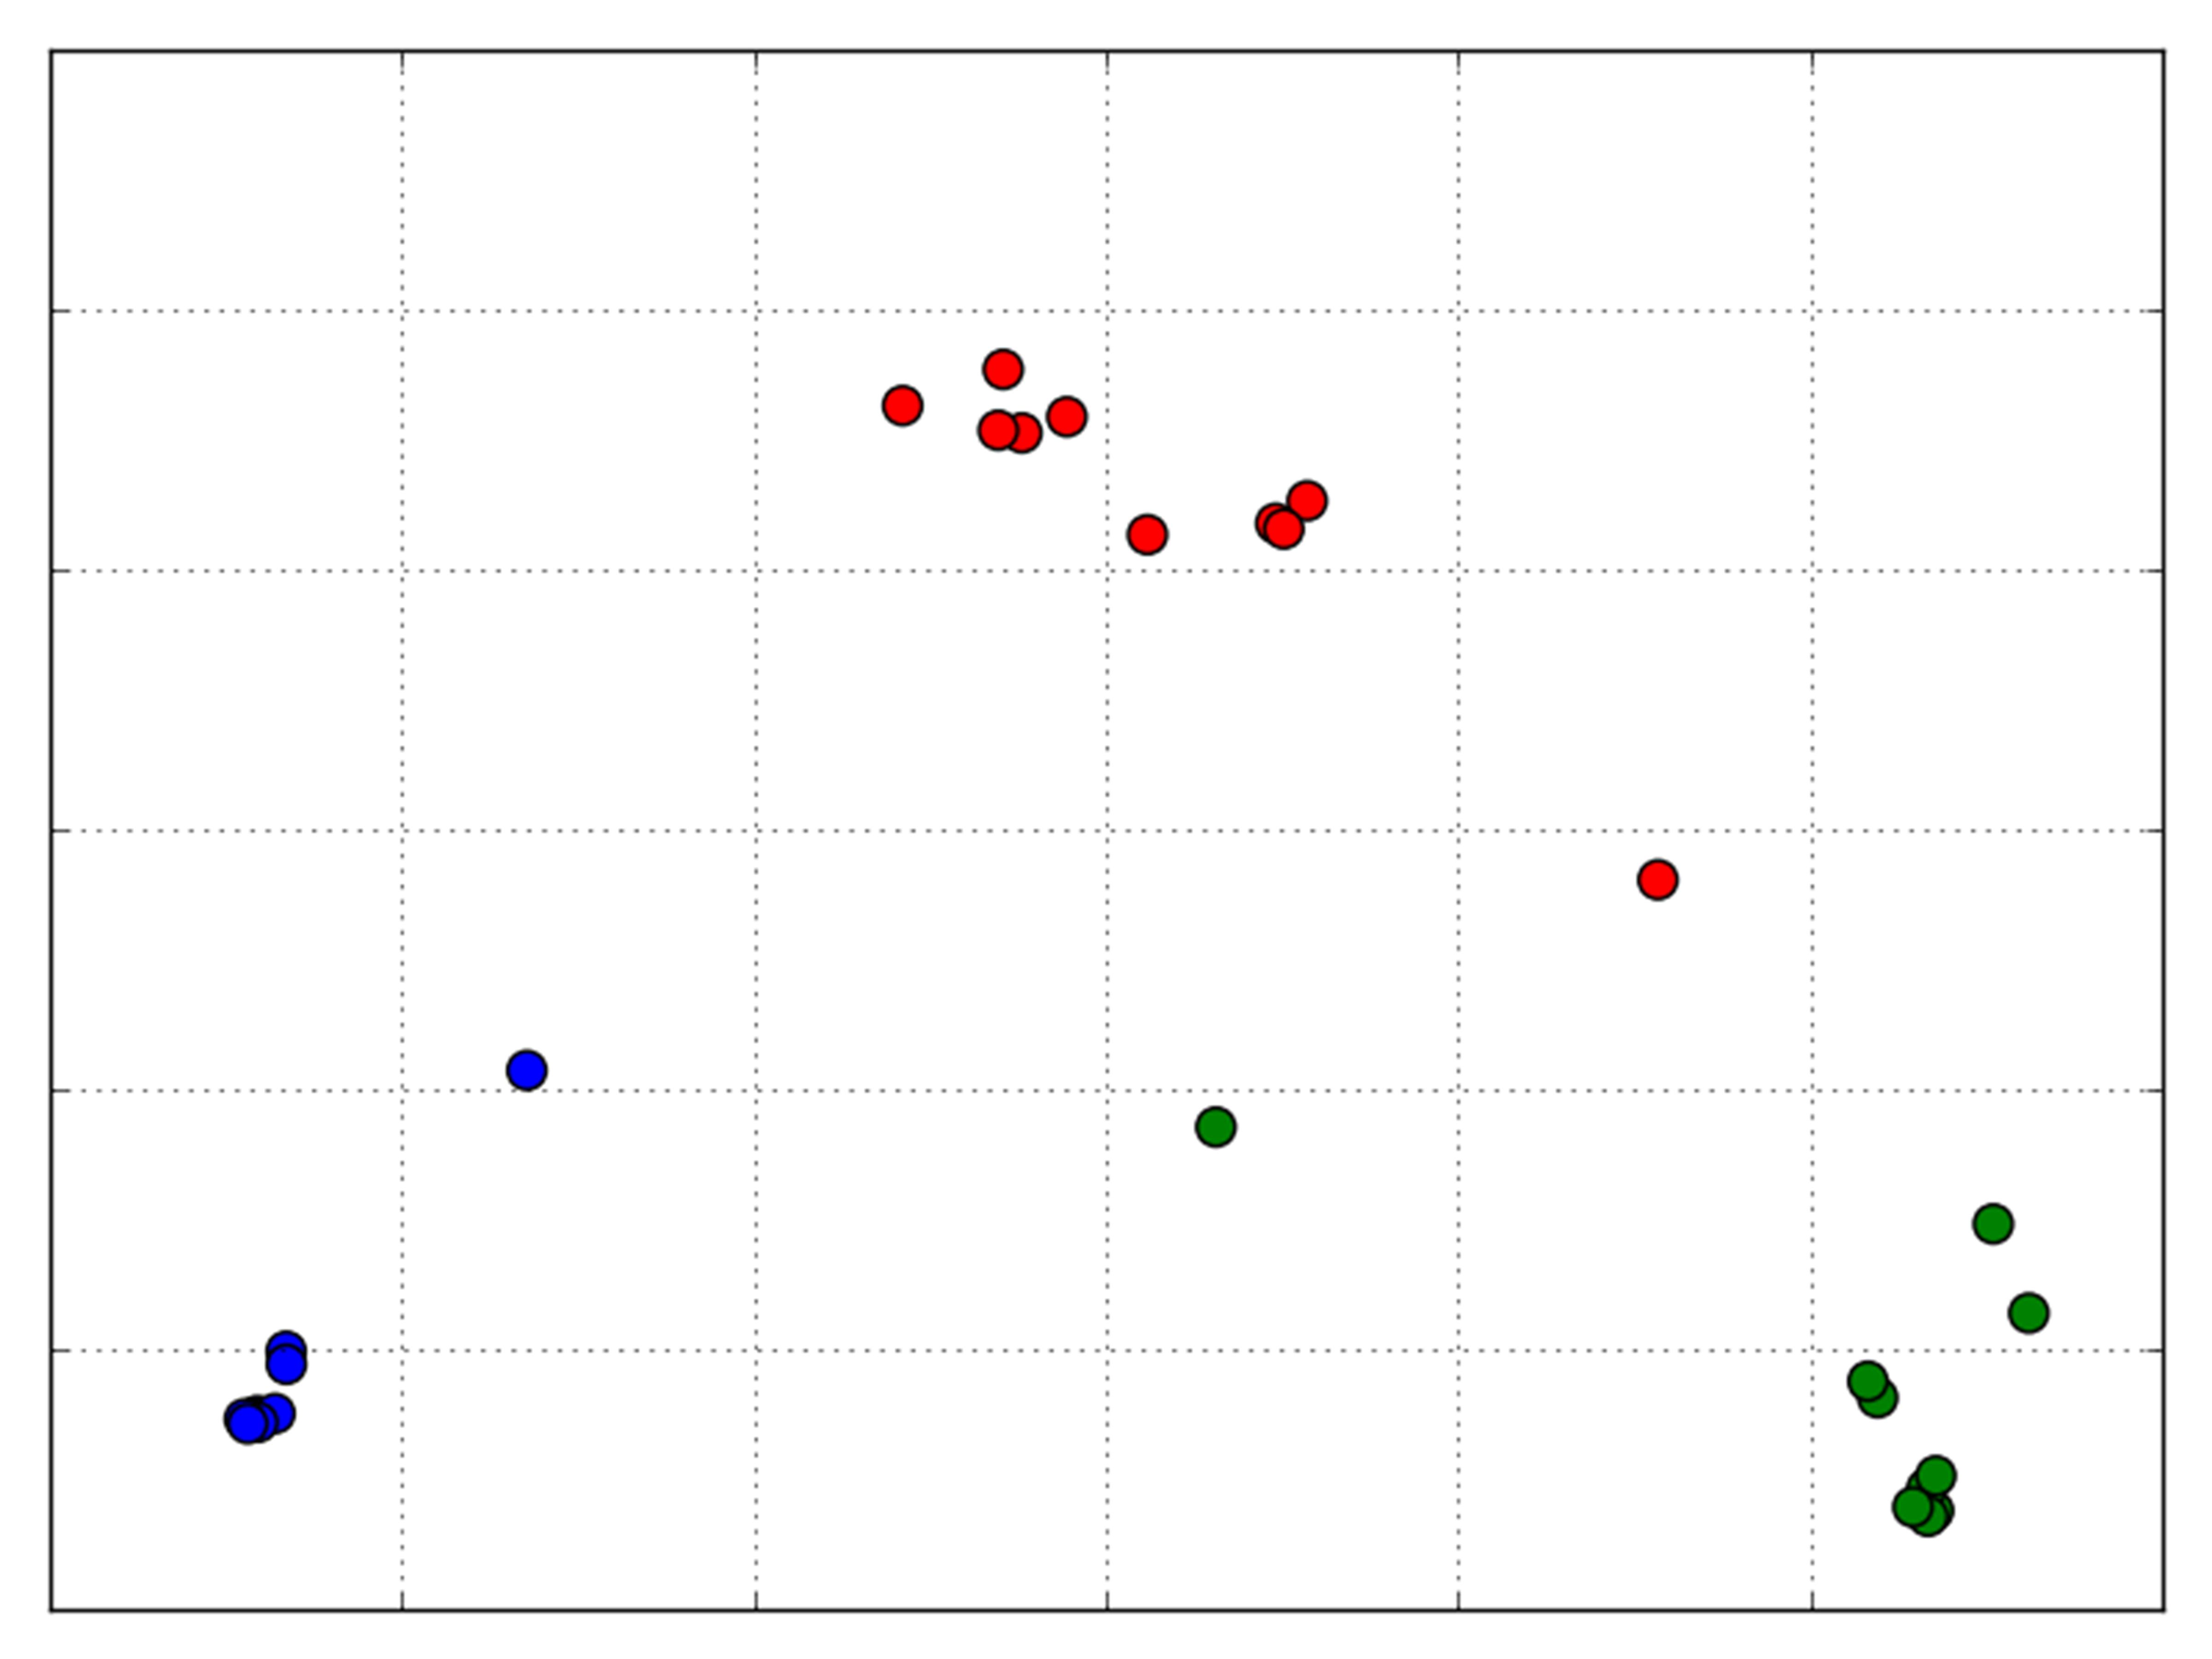
\includegraphics[width=.9\linewidth]{fig/results/context_vector2.png}
        \caption{5\% noise}
        \label{fig:context_vector_plot_5}
    \end{subfigure}
    \captionsetup{justification=centering}
    \caption{Encoded vector for three different words with applied noise}
    \label{fig:context_vector_plot}
\end{figure}

The plot can be seen in Figure \ref{fig:context_vector_plot}, where the three clusters are the words ``PYRAMIDS'' (red), ``MYTHIC'' (blue), and ``SNOWMAN'' (green). Figure \ref{fig:context_vector_plot_1} had 1\% noise applied, while Figure \ref{fig:context_vector_plot_5} had 5\% noise applied. Both figures show that the three words are clustered close to each other, while the plot with 5\% has the points scattered further apart with a few outliers. Figure \ref{fig:context_vector_plot_1} illustrates that despite some noise, the encoding retains the meaning of the word itself. The same is seen in Figure \ref{fig:context_vector_plot_5}, although the noise has made the encoding more indistinct and the points more scattered.

\subsection{Decoding}
The decoder and its ability to feed previous output back as input is one of the corner-stones i the encoder-decoder framework. Allowing the decoder to read the previous output helps the decoder know something about the current state of the ``translation'' process from the vector passed on from the encoder. If the decoder did not feed the output back as input, it would have to rely solely on the hidden and cell states for the decoding process.

\begin{figure}[!ht]
    \centering
    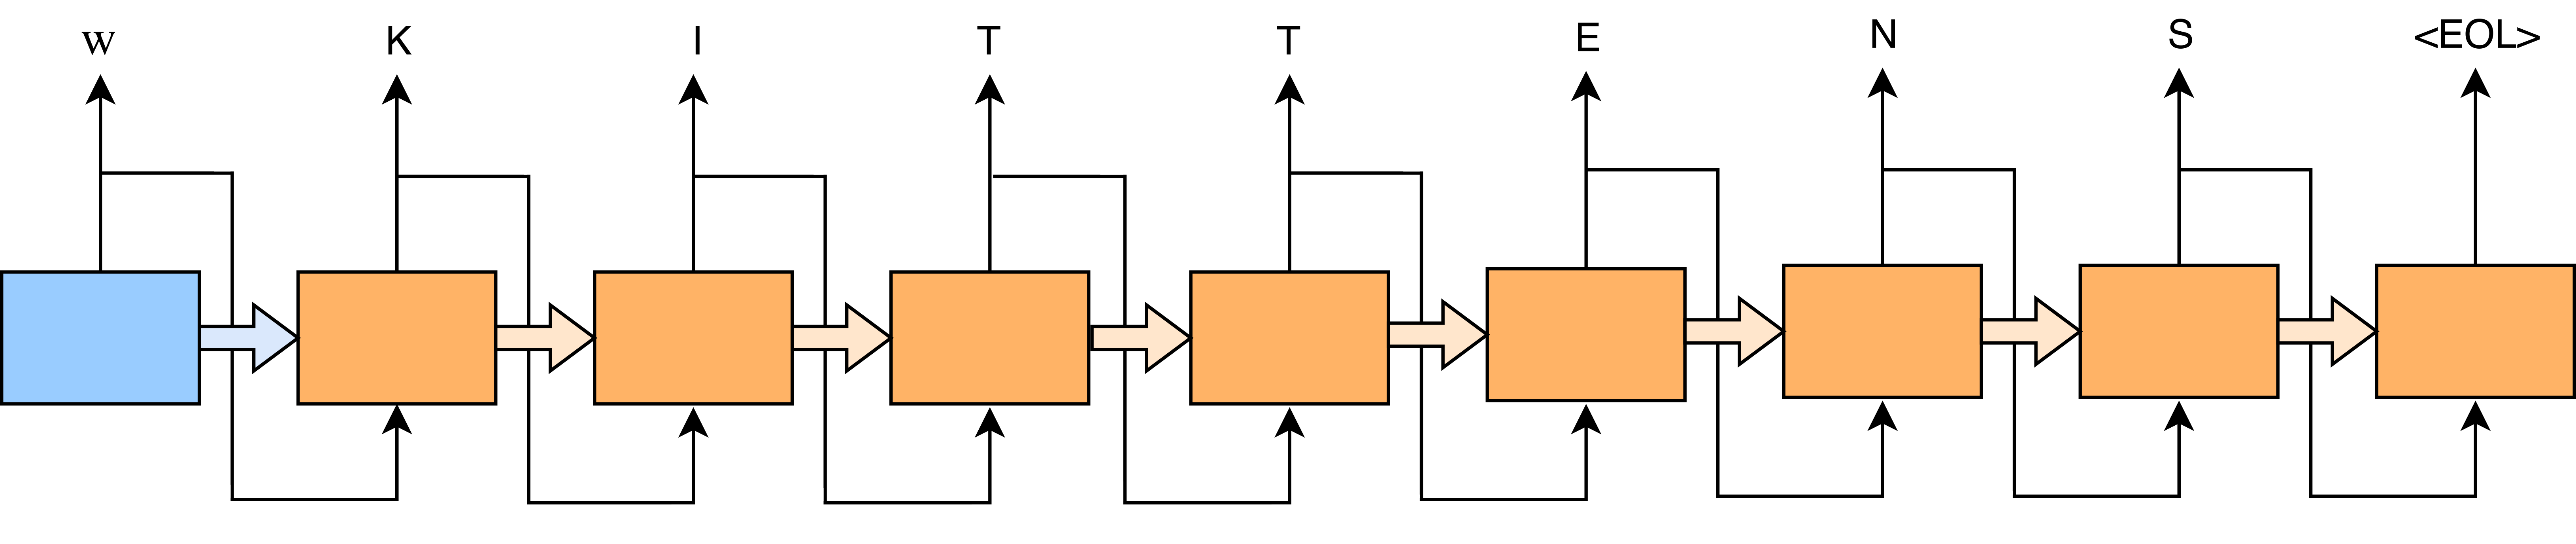
\includegraphics[width=1\textwidth]{fig/results/kittens_correct.png}
    \caption{Decoding the word ``KITTENS''}
    \label{fig:kittens_correct}
\end{figure}

During decoding, the decoder outputs a vector for each timestep, ran through a softmax function. The framework uses {\tt argmax} to find the element in the vector with the highest value, e.i. the predicted value, and feeds this value back to the decoder for the next timestep. Here we have altered this functionality, instead of feeding back the predicted value, we send something else back and see how the decoder reacts. Without any modification to the feedback-behavior, the model we used is perfectly able to classify each label in the word and produces the correct output ``KITTENS'', as illustrated in Figure \ref{fig:kittens_correct}. 

\begin{figure}[!ht]
    \centering
    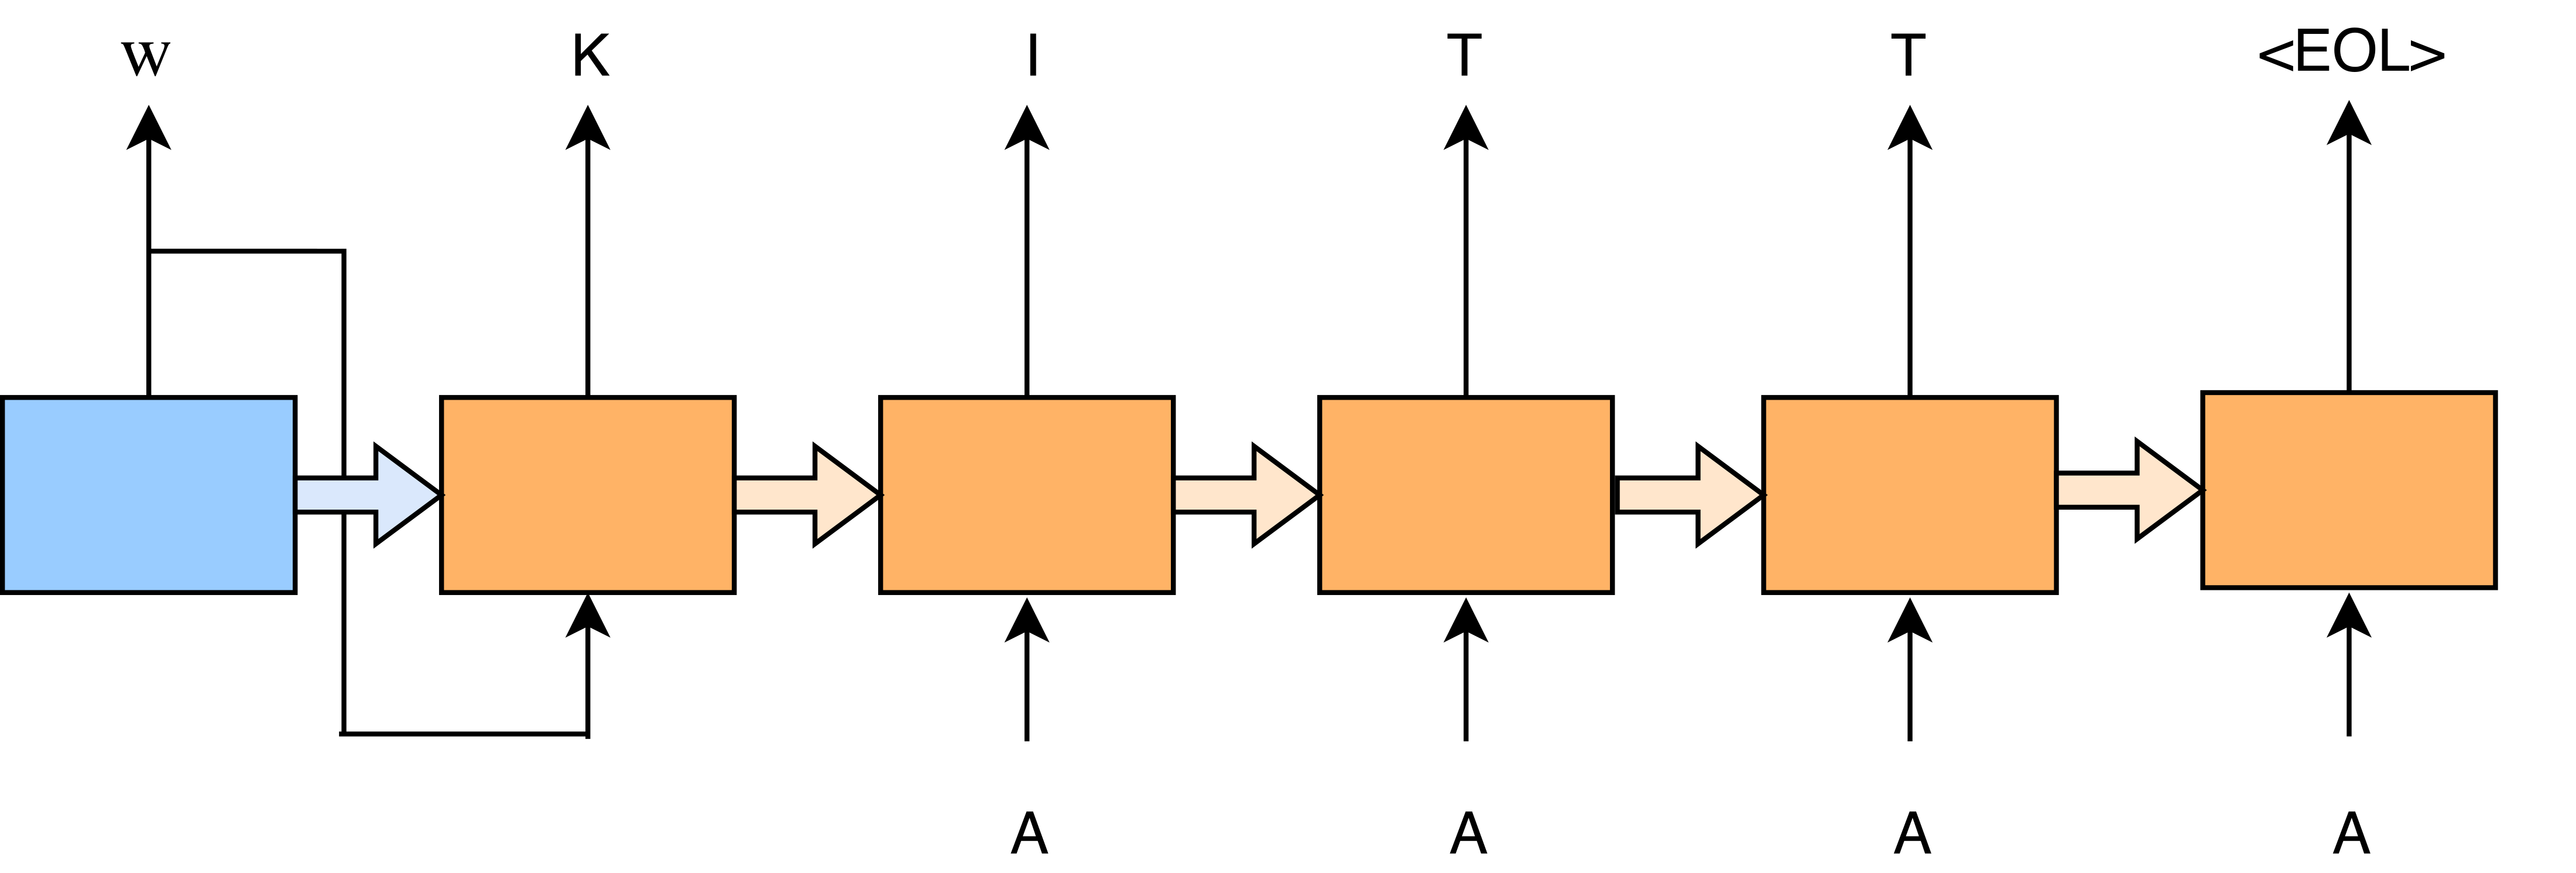
\includegraphics[width=1\textwidth]{fig/results/kittens_wrong.png}
    \caption{Decoding the word ``KITTENS'' by feeding back wrong label}
    \label{fig:kittens_wrong}
\end{figure}

If we instead change the logic to use the {\tt argmin} function, which returns the element we predicted the ``least'', the word becomes ``KIIIEES''. Similarly, if we only feed back the first label, which in this case would be the letter A, the word becomes ``KITTT'', as illustrated in Figure \ref{fig:kittens_wrong}. Note that the first letter in the word is predicted based on the context vector from the encoder, so it is likely this is correct. Except the first letter, we see some of the other letters in the word have changed. However, despite our trickery, the decoder is still able to predict labels that are actually in the word, indicating the some of the ``knowledge'' in the decoding process is also stored and shared within the LSTM cell. We also observe that the output is not that far off, with both the misled decoders outputting the second letter correctly. Lastly, if we only ``fool'' the decoder for the first and/or second letter, telling it we outputted an A, the decoder is able to predict each letter correctly, outputting ``KITTENS". This also indicates that the knowledge in the cell states may correctly override the input, instead of creating a ``domino'' effect like we first expected, where the output would progressively get more and more wrong.

These observations indicates that the encoded context vector contains partial knowledge about which labels to output, especially the first couple of labels. As the decoding progresses, the decoder shifts the attention more towards the previous output, and relies less on the information from the context vector.

\subsection{Use of Attention}
The experiments carried out in this thesis showed that both the models based on the encoder-decoder were powerful, but the model that utilized the attention mechanism was significantly better on the most complex experiment. Figure \ref{fig:attention_heatmap} shows the attention heatmap, in other words, the areas in which the attention mechanism focused while classifying each individual label. In this example the model correctly classifies the word ``IMAGINED'' without any errors. 

The heatmap shows how the attention mechanism scanned both the related input, as well as input ahead of time, making use of the additional data to do the classifications. Comparing the heatmap in Figure \ref{fig:attention_heatmap} with the actual text and signature in Figure  \ref{fig:imagine_highlighted}\footnote{In this illustration the white pixels are highlighted in green, and black pixels are highlighted in red}, we can see that the heatmap focus almost matches the related input areas for each label. This additional information gives the {\tt EncDecAtt} a significant advantage over the {\tt EncDecReg} model, which can only rely on the information in the context vector. We see that this benefit pays off in the consistently better results the {\tt EncDegAtt} model has compared to the {\tt EncDecReg}. The heatmap also show how the attention mechanism is able to keep attention fixed on longer subsequences, accounting for the different width ratio between input and output.

\begin{figure}[ht]
    \centering
    \includegraphics[width=1\textwidth]{fig/conclusion/attention_crop.png}
    \caption{Attention heatmap}
    \label{fig:attention_heatmap}
\end{figure}

\begin{figure}[ht]
    \centering
    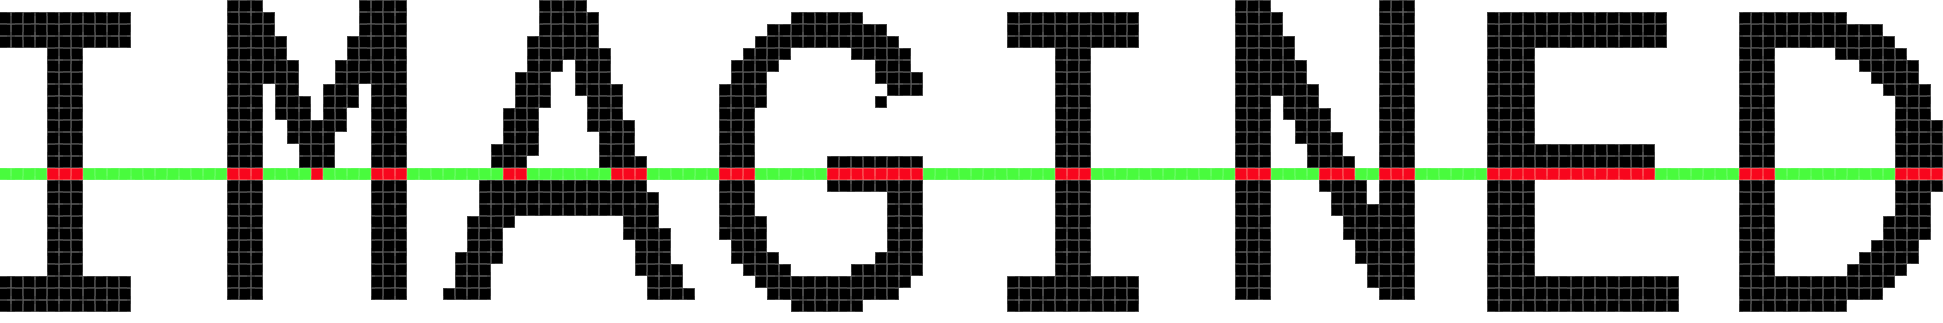
\includegraphics[width=1\textwidth]{fig/conclusion/imagined_grid_exported.png}
    \caption{The word ``IMAGINED'' with the signature highlighted in red and green}
    \label{fig:imagine_highlighted}
\end{figure}
